\documentclass[twoside,12pt]{ctexart}
% \documentclass[letterpaper]{article}

% Any additional packages needed should be included after jmlr2e.
% Note that jmlr2e.sty includes epsfig, amssymb, natbib and graphicx,
% and defines many common macros, such as 'proof' and 'example'.
%
% It also sets the bibliographystyle to plainnat; for more information on
% natbib citation styles, see the natbib documentation, a copy of which
% is archived at http://www.jmlr.org/format/natbib.pdf

\usepackage{jmlr2e}

% \usepackage{lastpage}
% \jmlrheading{23}{2022}{1-\pageref{LastPage}}{12/2021; Revised 10/2022}{12/2022}{21-0000}{Nikola Kovachki and Zongyi Li}


\usepackage{lastpage}
\jmlrheading{23}{2022}{1-\pageref{LastPage}}{12/21; Revised 10/22}{12/22}{21-1524}{ Nikola Kovachki, Zongyi Li, Burigede Liu, Kamyar Azizzadenesheli, Kaushik Bhattacharya, Andrew Stuart, Anima Anandkumar}
\ShortHeadings{Neural Operator: Learning Maps Between Function Spaces With Applications to PDEs}{ Kovachki,  Li,  Liu,  Azizzadenesheli,  Bhattacharya,  Stuart,  Anandkumar}


\firstpageno{1}

% \usepackage[margin=1in]{geometry}
\usepackage{breakcites}
\usepackage{natbib}
\usepackage{enumitem,kantlipsum}

\usepackage{booktabs}       % professional-quality tables
\usepackage{amsmath} 
%\usepackage{amsthm}
\usepackage{amsfonts,pifont}       % blackboard math symbols
\usepackage{mathtools}
\usepackage{nicefrac}       % compact symbols for 1/2, etc.
\usepackage{xcolor}
\usepackage{soul}
\usepackage{dsfont}
\usepackage{hyperref}
%\usepackage{enumerate}
\usepackage{tikz-cd}
\usepackage{subcaption}

\usepackage{graphicx}
% Set the typeface to Times Roman
\usepackage{times}
\usepackage{dsfont}

\usepackage{diagbox}

\newcommand{\one}{\mathds{1}}
\newcommand{\cmark}{\ding{51}}%
\newcommand{\xmark}{\ding{55}}%
\definecolor{darkred}{rgb}{.7,0,0}
\definecolor{darkgreen}{rgb}{0,.7,0}

\newcommand{\kamyar}[1]{\textcolor{red}{Kamyar:~#1}}
\newcommand{\nk}[1]{{\color{black}{#1}}}
\newcommand{\say}[1]{{\color{blue}{#1}}}
\newcommand{\ams}[1]{{\color{darkred}{#1}}}
%\newcommand{\as}[1]{{\color{darkred}{#1}}}
\newcommand{\as}[1]{{\color{black}{#1}}}
\newcommand{\zl}[1]{{\color{darkgreen}{#1}}}
\newcommand{\todo}[1]{{\color{darkgreen}{#1}}}
\newcommand{\done}[1]{{\iffalse \color{darkgreen}{#1} \fi}}
\newcommand{\postponed}[1]{{\iffalse \color{darkgreen}{#1} \fi}}
% \newcommand{\hold}[1]{{\iffalse \color{darkgreen}{#1} \fi}}
\newcommand{\hold}[1]{#1}


\newcommand{\A}{\mathcal{A}}
\newcommand{\N}{\mathbb{N}}
\newcommand{\Z}{\mathbb{Z}}
\newcommand{\bbZ}{\mathbb{Z}}
\newcommand{\R}{\mathbb{R}}
\newcommand{\C}{\mathbb{C}}
\newcommand{\E}{\mathbb{E}}
\newcommand{\U}{\mathcal{U}}

\newcommand{\LL}{\mathsf{L}}
\newcommand{\cR}{\mathcal{R}}
\newcommand{\cK}{\mathcal{K}}
\newcommand{\cP}{\mathcal{P}}
\newcommand{\cQ}{\mathcal{Q}}
\newcommand{\cW}{\mathcal{W}}

% F for the Fourier transform
% G for the target operator
\newcommand{\Ftrue}{\mathcal{G}^\dagger}
\newcommand{\G}{\mathcal{G}}
\newcommand{\F}{\mathcal{G}}
\newcommand{\Fd}{\mathcal{G}^{\dagger}}
\newcommand{\cFd}{\mathcal{G}^{\dagger}}
\newcommand{\cF}{\mathcal{G}}
\newcommand{\cG}{\mathcal{F}}


\newcommand{\K}{\mathbb{K}}
\newcommand{\X}{\mathcal{X}}
\newcommand{\Y}{\mathcal{Y}}
\newcommand{\Prb}{\mathbb{P}}
\newcommand{\idn}{\mathbbm{1}}
\newcommand{\Exp}{\mathbb{E}}
\newcommand{\NN}{\mathsf{N}}
\newcommand{\ds}{\:\text{d}\sigma}
\newcommand{\dx}{\:\mathsf{d}x}
\newcommand{\dy}{\:\mathsf{d}y}
\newcommand{\pD}{\partial \Omega}
\newcommand{\DN}{\mathcal{F}}


\DeclareMathOperator*{\argmax}{arg\,max}
\DeclareMathOperator*{\argmin}{arg\,min}

\DeclarePairedDelimiter{\ceil}{\lceil}{\rceil}


\newtheorem{assumption}[theorem]{Assumption}

\newcommand{\vdown}{\check{v}}
\newcommand{\vup}{\hat{v}}
\newcommand{\eps}{\epsilon}

% \newtheorem{definition}{Definition}
% \newtheorem{theorem}{Theorem}
% \newtheorem{lemma}[theorem]{Lemma}
% \newtheorem{proposition}[theorem]{Proposition}
% \newtheorem{remark}{Remark}


\begin{document}

\title{
% Graph Kernel Network for Partial Differential Equations\\
% Graph Kernel Network As Inverse of Differential Operator\\
% Neural Operator: Neural Networks For \\
% Maps Between Function Spaces\\
Neural Operator: Learning Maps Between Function Spaces \\ With Applications to PDEs
% Deep Graph Kernel Networks for Infinite Dimensional Mappings?
}



\renewcommand{\thefootnote}{\fnsymbol {footnote}}

% \author{\name Nikola Kovachki\thanks{Equal contribution.} \,\thanks{Majority of the work was completed while the author was at Caltech.} \email nkovachki@nvidia.com \addr Nvidia
% \AND \name Zongyi Li$^*$ \email zongyili@caltech.edu \addr Caltech
% \AND \name Burigede Liu \email bl377@cam.ac.uk \addr Cambridge University
% \AND \name Kamyar Azizzadenesheli \email kamyara@nvidia.com \addr  Nvidia
% \AND \name Kaushik Bhattacharya \email bhatta@caltech.edu \addr Caltech
% \AND \name Andrew Stuart \email astuart@caltech.edu \addr Caltech
% \AND \name Anima Anandkumar \email anima@caltech.edu \addr Caltech
% }

% \author{Nikola Kovachki$^*$, Zongyi Li\footnote{equal contribution}, Burigede Liu,\\Kamyar Azizzadenesheli,
% Kaushik Bhattacharya,  Andrew Stuart, Anima Anandkumar}
% \date{\today}

% The author names and affiliations should appear only in the accepted paper.
%
%\author{ {\bf Harry Q.~Bovik\thanks{Footnote for author to give an
%alternate address.}} \\
%Computer Science Dept. \\
%Cranberry University\\
%Pittsburgh, PA 15213 \\
%\And
%{\bf Coauthor}  \\
%Affiliation          \\
%Address \\
%\And
%{\bf Coauthor}   \\
%Affiliation \\
%Address    \\
%(if needed)\\
%}
% \newcommand{\kamyar}[1]{\textcolor{red}{#1}}

% \editor{Lorenzo Rosasco}

% \maketitle
\tableofcontents

\begin{abstract}

神经网络的经典发展主要聚焦于学习有限维欧几里得空间或有限集合之间的映射。我们提出将神经网络推广至算子学习领域,这类算子被称为 “神经算子”(neural operators),可在无限维函数空间之间实现映射。
我们将神经算子表述为由线性积分算子与非线性激活函数构成的组合。针对所提神经算子,我们证明了其满足通用逼近定理 —— 这表明它能够逼近任意给定的非线性连续算子。此外,所提神经算子还具有离散化不变性:即在底层函数空间的不同离散化形式下,它们可共享相同的模型参数。
同时,我们提出了四类高效参数化方法,即图神经算子(graph neural operators)、多极图神经算子(multi-pole graph neural operators)、低秩神经算子(low-rank neural operators)以及傅里叶神经算子(Fourier neural operators)。
神经算子的一个重要应用场景是为偏微分方程(PDE)求解算子学习替代映射。我们以伯格斯方程(Burgers)、达西地下水流方程(Darcy subsurface flow)和纳维 - 斯托克斯方程(Navier-Stokes equations)等标准 PDE 为研究对象,结果表明:所提神经算子相较于现有基于机器学习的方法具有更优性能,同时其速度比传统 PDE 求解器快数个数量级。

The classical development of neural networks has primarily focused on learning mappings between finite dimensional Euclidean spaces or finite sets.
We propose a generalization of neural networks to learn operators, termed \emph{neural operators}, that map between infinite dimensional function spaces.
We formulate the neural operator as a composition of  linear integral operators and nonlinear activation functions. We prove a universal approximation theorem for our proposed neural operator, showing that it can approximate any given nonlinear continuous operator. The proposed neural operators are also discretization-invariant, i.e., they share the same model parameters among different discretization of the underlying function spaces. 
Furthermore, we introduce four classes of efficient parameterization, viz., graph neural operators,  multi-pole graph neural operators, low-rank neural operators, and Fourier neural operators.
An important application for neural operators is learning surrogate maps for the solution operators of
partial differential equations (PDEs). We consider standard PDEs such as the Burgers, Darcy subsurface flow, and the Navier-Stokes equations, and show that the proposed neural operators have superior performance compared to existing machine learning based methodologies,
while being several orders of magnitude faster than conventional PDE solvers. 

%Numerical experiments are presented in which the solution operator (mapping initial condition to solution)  is learned for Burgers' equation and the Navier-Stokes equation, and in which the coefficient to solution map is learned in the Darcy model of porous medium flow; a variety of linear operators, defined by linear  PDEs, are also used to illustrate key ideas.



% \kamyar{
% The classical development of neural networks has been primarily for mappings between a finite-dimensional spaces, e.g., between Euclidean space and a set of classes/labels, or between two finite-dimensional Euclidean spaces.
% The purpose of this work is to generalize neural networks so that they can learn operators mapping between general spaces, e.g., between infinite dimensional spaces, such as function spaces. 
% We formulate the approximation of operators by composition of nonlinear local activation functions and a class of linear local and non-local integral operators, so that the composed operator can approximate complex nonlinear, local, and non-local operators.
% In this paper, we propose four formulations of the integral operators: graph-based operators, multipole graph-based operators, low rank operators, and Fourier operators.
% Experiments confirm that the proposed neural operators have the desirable resolution-invariant properties and show competitive performance compared to existing methodologies from both the fields of neural networks and numerical analysis. }
 
\end{abstract}

\begin{keywords}
  Deep Learning, Operator Learning, Discretization-Invariance, Partial Differential Equations, Navier-Stokes Equation.
\end{keywords}

%%%%%%%%%%%%%%%%%%%%%%%%%%%%%%%%%%%%%%%%%%%%%%%%%%%%
%
%  Introduction
%
%%%%%%%%%%%%%%%%%%%%%%%%%%%%%%%%%%%%%%%%%%%%%%%%%%%%





\section{Introduction}
\label{sec:I}
% 学习此类映射的可能性,为设计具有广泛适用性的深度学习框架开辟了一类新问题。传统神经网络是有限维欧氏空间(finite-dimensional Euclidean spaces)和 / 或有限基数集合(sets of finite cardinality)之间的映射,基于传统神经网络进行拓展需要新的思路。这涉及无穷维空间(infinite-dimensional spaces),例如输入和输出本身是定义在欧氏空间某一区域上的函数的情况。
学习函数空间(function spaces)之间的映射在科学与工程领域具有广泛应用。例如,在求解微分方程(differential equations)时,输入为系数函数(coefficient function),输出为解函数(solution function)。解决该问题的一种直接方法是将无穷维的输入和输出函数空间离散化(discretize)为有限维网格(finite-dimensional grids),并应用神经网络(neural networks)等标准学习模型。然而,这种方法会限制适用性,因为所学习的神经网络模型可能无法很好地泛化到训练数据离散化网格(discretization grid)之外的其他离散化(discretizations)情况。
为克服标准神经网络的这些局限性,我们构建(formulate)了一个用于学习算子的新型深度学习框架,称为 {\em 神经算子(neural operators)},它可直接在有界区域(bounded domains)上的函数空间之间进行映射。由于我们的神经算子是在函数空间上设计的,因此可以通过多种不同方法、在不同分辨率(resolution)水平下对其进行离散化,且无需重新训练。相比之下,标准神经网络架构严重依赖训练数据的离散化:对于不同离散化程度的数据,可能需要具有新参数的新架构才能达到相同的误差水平。我们还提出了 {\em 离散化不变(discretization-invariant)} 模型的概念(notion),并证明我们的神经算子满足该性质(property),而标准神经网络则不满足。
% 此类神经算子模型一旦训练完成,便具有离散化不变性质:可在基础函数数据的不同离散化形式之间共享相同的模型参数。我们通过数值实验证明,对于数据的任意离散化形式,同一神经算子都能实现低误差,而标准前馈神经网络(feed-forward neural networks)和卷积神经网络(convolutional neural networks)则无法做到。在偏微分方程(partial differential equations, PDEs)场景下,我们通过数值实验证明,在固定分辨率下,所提出的方法与神经网络模型相比具有很强的竞争力,且比用于生成数据的偏微分方程求解器(PDE solvers)快几个数量级(orders of magnitude)。
% 最后,我们为所提出的神经算子建立了通用逼近定理(universal approximation theorem),证明它们能够以任意精度逼近线性和非线性算子(linear and non-linear operators)。
% 本文研究了偏微分方程模型衍生的各类解算子(solution operators)或流映射(flow maps);具体而言,我们研究了函数空间之间的映射,其中输入数据例如可以是初始条件(initial condition)、边界条件(boundary condition)或系数函数,而输出数据则是相应的解。我们针对以下算子开展了数值实验:一维泊松方程(one-dimensional Poisson equation)\citep {Evans}、一维时间相关伯格斯方程(time-dependent one-space-dimensional Burgers' Equation)\citep {Evans}、二维稳态达西流动(two-dimensional steady Darcy Flow)\citep {bear2012fundamentals} 以及二维时间相关不可压缩纳维 - 斯托克斯方程(time-dependent two-space dimensional incompressible Navier-Stokes Equation)\citep {constantin1988navier,lemarie2018navier,temam2001navier}。
%3.1 节(Subsection \ref {ssec:LR})介绍了本文工作的研究背景与相关背景信息。3.2 节(Subsection \ref {ssec:OC})详细阐述了我们的研究贡献,并概述了论文内容。本文引言部分在 3.3 节(Subsection \ref {ssec:related-work})结束,该节提供了文献综述(literature review)。

%The possibility of learning such mappings opens up a new class of problems in the design of deep learning frameworks with widespread applicability. New ideas are required to build upon traditional neural networks which are mappings between finite-dimensional Euclidean spaces and/or sets of finite cardinality.   This involves infinite-dimensional spaces, such as the case where inputs and outputs are themselves functions over a domain in the Euclidean space

Learning mappings between  function spaces has widespread applications  in science and engineering. For instance, for  solving differential equations,  the input is a coefficient function and the output is a solution function. A straightforward solution to this problem  is to simply  discretize the infinite-dimensional input and output function spaces into finite-dimensional grids, and apply standard learning models such as 
neural networks. However, this limits  applicability since the learned  neural network model may not  generalize well to different discretizations, beyond the discretization grid of the training data.

To overcome these limitations of standard neural networks, we  formulate a new deep-learning framework for learning operators, called {\em neural operators}, which directly map between  function spaces on bounded domains.  Since our neural operator is  designed on function spaces, they
can be discretized by a variety of different methods, and at different levels of resolution, without the need for re-training. In contrast, standard neural network architectures depend heavily on the discretization of training data: new architectures with new parameters may be needed to achieve the same error for   data with varying discretization.  We also propose the notion of {\em discretization-invariant} models and prove that our neural operators satisfy this property, while standard neural networks do not. 

%Such neural operator models, once trained, have the  property of being  discretization invariant: it is possible to share the same model parameters among different discretization of the underlying functional data. We demonstrate, numerically, that the same neural operator can achieve a low error for any discretization of the data while standard feed-forward and convolutional neural networks cannot. In the context of partial differential equations (PDEs) we demonstrate numerically that, at fixed resolution, the resulting methods are highly competitive when compared with neural network models and are orders of magnitude faster than the PDE solvers used to generate data. 

%Finally we establish a universal approximation theorem for the neural operators we introduce, proving their ability to approximate linear and non-linear operators arbitrary well.

%In this paper we study various solution operators or flow maps arising from PDE models; in particular, we investigate  mappings between function spaces where the input data can be, for example, the initial condition, boundary condition, or coefficient function, and the output data are the respective solutions. We perform numerical experiments with operators arising from the one-dimensional Poisson equation \citep{Evans}, the time-dependent one-space-dimensional Burgers' Equation \citep{Evans},  two-dimensional steady Darcy Flow \citep{bear2012fundamentals} and the time-dependent two-space dimensional incompressible Navier-Stokes Equation \citep{constantin1988navier,lemarie2018navier,temam2001navier}.

%Subsection \ref{ssec:LR} contains background and context for our work. Subsection \ref{ssec:OC} details our contributions and outlines the contents of the paper. We conclude this introduction in Subsection \ref{ssec:related-work} which provides a literature review. 


\subsection{Our Approach}
\label{ssec:OC}



\paragraph{Discretization-Invariant Models.}

We formulate a precise mathematical notion of discretization invariance. We require any discretization-invariant model with a fixed number of parameters to satisfy the following:
\begin{enumerate}[leftmargin=*]
    \item  acts on any discretization of the input function, i.e. accepts any set of points in the input domain,
    \item can be evaluated at any point of the output domain,
    \item  converges to a continuum operator as the discretization is refined. 
\end{enumerate} 



\noindent The first two requirements of accepting any input and output points in the domain is a natural requirement for discretization invariance, while the last one ensures consistency in the limit as the discretization is refined. For example, families of graph neural networks~\citep{scarselli2008graph} and transformer models~\citep{vaswani2017attention} are resolution invariant, i.e., they can receive inputs at any resolution, but they fail to converge to a continuum operator as discretization is refined. Moreover, we require the models to have a fixed number of parameters; otherwise, the number of parameters becomes unbounded in the limit as the discretization is refined, as shown in Figure \ref{fig:discretization-invariance}.  Thus the notion of discretization invariance allows us to define neural operator models that are consistent in function spaces and can be applied to data given at any resolution and on any mesh. We also establish that standard neural network models are not discretization invariant.

% \todo{zongyi: can u add fig for mesh refinement for air foil. it is fine that it is irregular. we are defining notion here. }

%\begin{figure}[h]
%\includegraphics[width=\textwidth]{}
%\end{figure}



\begin{figure}[h]
    \centering
    \includegraphics[width=0.8\textwidth]{Figs/discretization-invariance.png}
    \caption{Discretization Invariance}
    \label{fig:discretization-invariance}
    An discretization-invariant operator has convergent predictions on a mesh refinement.
\end{figure}

\paragraph{Neural Operators.}


We introduce the concept of neural operators   for learning operators that are  mappings between infinite-dimensional function spaces. We propose neural operator architectures to be multi-layers where layers  are themselves operators composed with non-linear activations. This ensures that that the overall end-to-end composition  is an operator, and thus satisfies the discretization invariance property. The key design choice for neural operator is the operator layers. To keep it simple, we limit ourselves to layers that are linear operators. Since these layers are composed with non-linear activations, we obtain neural operator models that are expressive and able to capture any continuous operator. The latter property is known as universal approximation. 

The above line of reasoning for neural operator design follows closely the design of standard neural networks, where linear layers (e.g. matrix multiplication, convolution) are composed with non-linear activations, and we have universal approximation of continuous functions defined on compact domains~\citep{hornik1989multilayer}. Neural operators replace finite-dimensional linear layers in neural networks with linear operators in function spaces.


%We further show that neural operators models are universal approximators of operators acting between Banach spaces. It is well known that neural networks are universal approximators of functions, meaning that they can uniformly approximate any continuous function defined on a compact domain~\citep{hornik1989multilayer}. We analogously show that neural operators can uniformly approximate any continuous operator defined on a compact set of a Banach space. 
%Due to the generality of neural operators, it is desirable to study whether neural operators can approximate any operator. 

%\begin{theorem}[Universal approximation of operators]
%\label{thm:univ_approx_informal}
%Neural operators are universal approximators of operators. Given proper input and output function spaces, neural operators approximate any operator arbitrary accurately on an appropriate topology.
%\end{theorem}
%The formal statements of this, and related theorems, are provided in Subsection~\ref{sec:approximation_main}; proofs are in an appendix. %This theorem express that when using neural operators to approximate an operator in practice, one may not be concerned with the capacity of the model class from the approximation theoretic point of view. 



%\paragraph{Properties of Neural Operators.}


%\begin{theorem}[Discretization invariance of neural operators]
%\label{thm:disc_inv_informal}
%Neural operators satisfy the above criteria of being discretization-invariant and a fixed neural operator model can act on any discretization used to represent the input function. 
%\end{theorem}
%The formal statement of this theorem is provided in Subsection~\ref{sec:discritizational_invariance} with related discussion in Section~\ref{sec:neuraloperators}. 
%In this paper, we show that traditional neural networks are not discretization invariant models, while slightly modified transformers are resolution invariant models. 




We  formally establish that neural operator models with a fixed number of parameters satisfy discretization invariance. We further show that neural operators models are universal approximators of continuous operators acting between Banach spaces, and  can uniformly approximate any continuous operator defined on a compact set of a Banach space.   {\bf Neural operators are the only known class of models that guarantee both discretization-invariance and universal approximation.} See Table~\ref{table:deeplearning_comparison} for a comparison among the deep learning models. Previous deep learning models are mostly defined on a fixed grid, and  removing, adding, or moving grid points generally makes these models no longer applicable. Thus, they are  not discretization invariant. 


We propose several design choices for the linear operator layers in neural operator such as a parameterized integral operator or through multiplication in the spectral domain as shown in Figure~\ref{fig:NO_architecture}.  
Specifically, we propose four practical methods for implementing the neural operator framework: graph-based operators, low-rank operators, multipole graph-based operators, and Fourier  operators. Specifically, for graph-based operators, we develop a Nystr\"om extension to connect the integral operator formulation of the neural operator to families of graph neural networks (GNNs) on arbitrary grids. For Fourier operators,  we consider the spectral domain formulation of the neural operator which leads to efficient algorithms in settings where fast transform methods are applicable. 

We include an exhaustive numerical study of the four formulations of neural operators. Numerically, we show that the proposed methodology consistently outperforms all existing deep learning methods even on the resolutions for which the standard neural networks were designed. For the two-dimensional Navier-Stokes equation, when learning the entire flow map,  the method achieves $<1\%$ error for a Reynolds number of 20 and $8\%$ error for a Reynolds number of 200.

The proposed Fourier neural operator (FNO) has an inference time that is three orders of magnitude faster than the pseudo-spectral method used to generate the data for the Navier-Stokes problem \citep{chandler2013invariant} -- $0.005$s compared to the $2.2s$ on a $256 \times 256$ uniform spatial grid. %\todo{need to change this}
Despite its tremendous speed advantage, the method does not suffer from accuracy degradation when used in downstream applications such as solving Bayesian inverse problems. Furthermore, we demonstrate
that FNO is robust to noise on the testing problems we consider here.

\begin{figure}[t]
    \centering
    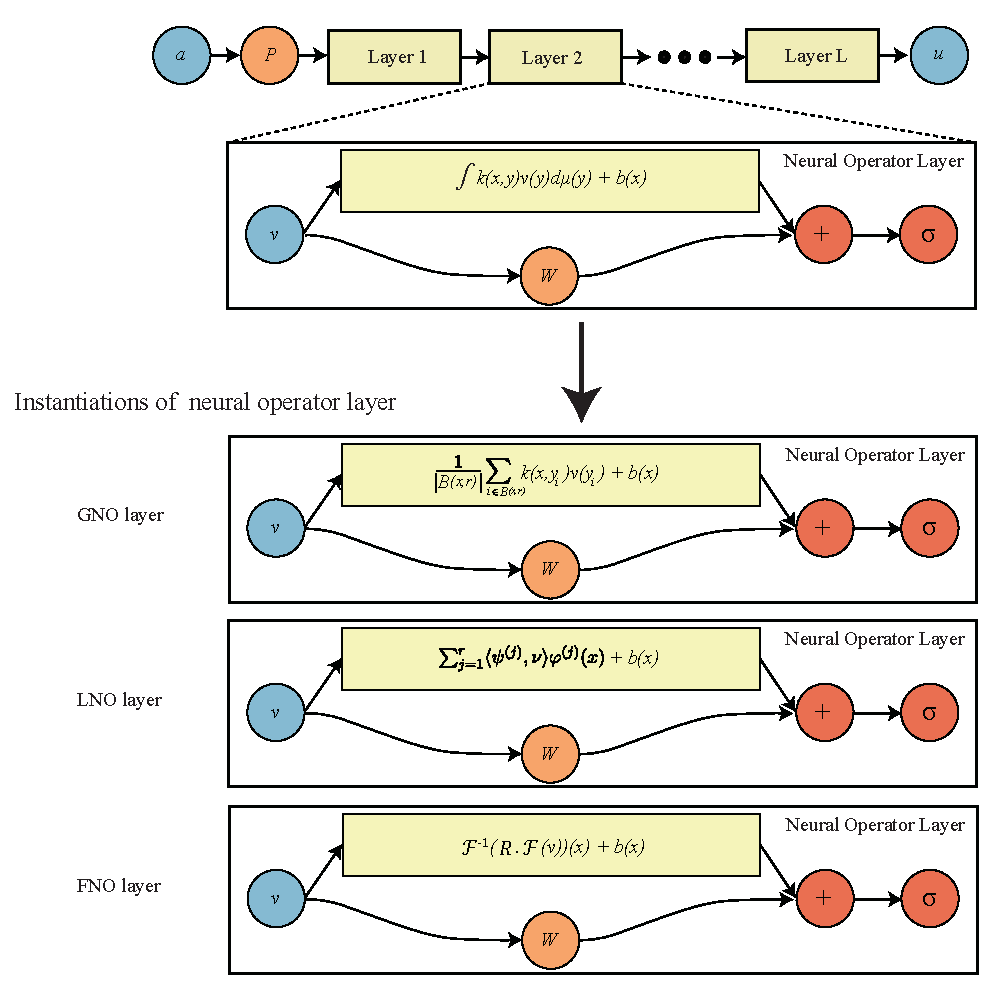
\includegraphics[width=0.8\textwidth]{Figs/NO-all-eq.pdf}
    \caption{Neural operator architecture schematic}
    \label{fig:NO_architecture} 
    \small{The input function $a$ is passed to a pointwise lifting operator $P$ that is followed by $T$ layers of integral operators and pointwise non-linearity operations $\sigma$. In the end, the pointwise projection operator $Q$ outputs the function $u$. Three instantiation of neural operator layers, GNO, LNO, and FNO are provided.}
\end{figure}



%This is undesirable since, in many scientific and engineering applications, function evaluations are often sensory and provided on varying per-sample grid points. In contrast, the discretization property of neural operators allows them to be defined and operator on varying grid locations and sizes, desirable characteristics for the downstream tasks. 


% \begin{table}[h!]
% \centering
% \begin{tabular}{l|c|c|c|c}
% % \diaghead{Scoreexp}{Property}{Model}&
% \diagbox{Property\hspace{.5cm}}{\hspace{2em}\raisebox{-.3cm}{Model}}&
% CNNs& DeepONets & Interpolation & Neural Operators\\
% \hline
% Discretization Invariance & \xmark & \xmark & \cmark & \cmark \\
% \hline
% Can the output function be queried at any point? & \xmark & \cmark & \cmark & \cmark \\
% \hline
% Input at any point & \nk{\cmark} & \xmark & \cmark & \cmark \\
% \hline
% Universal Approximation & \xmark & \cmark & \xmark & \cmark \\
% \hline
% \end{tabular}
% \caption{Comparison of deep learning models. The first row indicates whether the model is discretization invariant. The second and third rows indicate whether the output and input are a functions. The fourth row indicates whether the model class is a universal approximator of operators. Neural Operators are discretization invariant deep learning methods that output functions and can approximate any operator.}
% \label{table:deeplearning_comparison}
% \end{table}
% }


\begin{table}[h!]
\centering
\begin{tabular}{l|c|c|c|c}
% \diaghead{Scoreexp}{Property}{Model}&
\diagbox{Property\hspace{.5cm}}{\hspace{2em}\raisebox{-.3cm}{Model}}&
NNs& DeepONets & Interpolation & Neural Operators\\
\hline
Discretization Invariance & \xmark & \xmark & \cmark & \cmark \\
\hline
Is the output a function? & \xmark & \cmark & \cmark & \cmark \\
\hline
Can query the output at any point? & \xmark & \cmark & \cmark & \cmark \\
\hline
Can take the input at any point? & \nk{\xmark} & \xmark & \cmark & \cmark \\
\hline
Universal Approximation & \xmark & \cmark & \xmark & \cmark \\
\hline
\end{tabular}
\caption{Comparison of deep learning models. The first row indicates whether the model is discretization invariant. The second and third rows indicate whether the output and input are a functions. The fourth row indicates whether the model class is a universal approximator of operators. Neural Operators are discretization invariant deep learning methods that output functions and can approximate any operator.}
\label{table:deeplearning_comparison}
\end{table}



\subsection{Background and Context}
\label{ssec:LR}


\paragraph{Data-driven approaches for solving PDEs.}
%``Differential equations [...] represent the most powerful tool humanity has ever created for making sense of the material world.'' \citet{strogatz2009loves}. 
% A wide range of important engineering and physics problems are governed by PDEs. 
Over the past decades, significant progress has been made in formulating \citep{gurtin1982introduction} and solving \citep{johnson2012numerical} the governing PDEs in many scientific fields from micro-scale problems (e.g., quantum and molecular dynamics) to macro-scale applications (e.g., civil and marine engineering). Despite the success in the application of PDEs to solve real-world problems,  two significant challenges remain: (1) identifying the governing model for complex systems; (2) efficiently solving large-scale nonlinear systems of equations.

Identifying and formulating the underlying PDEs appropriate for modeling a specific problem usually requires extensive prior knowledge in the corresponding field which is then combined with universal conservation laws to design a predictive model. For example, modeling the deformation and failure of solid structures requires detailed knowledge of the relationship between stress and strain in the constituent material. For complicated systems such as living cells, acquiring such knowledge is often elusive and formulating the governing PDE for these systems remains prohibitive, or the models
proposed are too simplistic to be informative. The possibility of acquiring such knowledge from data can revolutionize these fields. 
Second, solving complicated nonlinear PDE systems (such as those arising in turbulence and plasticity) is computationally demanding and can often make realistic simulations intractable. Again the possibility of using instances of data to design fast approximate solvers holds great potential for accelerating numerous problems.

\iffalse
\subsection{Learning the Operator} We want to stress that learning the operator $\F$ is a more challenging task compared to finding the solution $u$ for a single equation. Most of the existing methods, ranging from traditional finite element methods (FEM), finite difference methods (FDM), to machine learning based physics-informed neural networks (PINNs) \citep{raissi2019physics}, they all aim to find $u$ for a single equation (i.e., single solving for a single $a$). On the other hand, we want to parameterize $\F$ as a mapping from $a\in\A$ to $u\in\U$.

Compared to PDE solvers such as FEM and PINNs, the neural operator learns the solution operator doesn't require to solve each equation separately. It immediately outputs the evaluation for any new query $a$. Therefore, it is usually used as a fast evaluator. For example, for inverse problem when one need to find some optimal material structures $a$, the neural operator can quickly evaluate input $a'$, combining with optimization methods to find $a' \to a$.
\fi 

\paragraph{Learning PDE Solution Operators.}
 In PDE applications, the governing differential equations are by definition local, whilst the solution operator exhibits non-local properties. Such non-local effects can be described by integral operators explicitly in the spatial domain, or by means of spectral domain multiplication; convolution is an archetypal example. For integral equations, the graph approximations of Nystr\"om type \citep{belongie2002spectral} provide a consistent way of connecting different grid or data structures arising in computational methods and understanding their continuum limits \citep{von2008consistency,trillos2018variational,trillos2020error}. For spectral domain calculations, there are well-developed tools that exist for approximating the continuum \citep{boyd2001chebyshev,trefethen2000spectral}. However, these approaches for approximating integral operators are not data-driven.  Neural networks present a natural approach for learning-based integral operator approximations since they can incorporate non-locality. However, standard neural networks are limited to the discretization of training data and hence, offer a poor approximation to the integral operator. We tackle this issue here by proposing the framework of neural operators. 
 
 %This is the governing principle underlying our work aimed at designing mesh invariant neural network approximations for the solution operators of PDEs.
 
 %Supervised learning has the potential to address these challenges when designed in a way that allows for the emulation of mappings between function spaces \citep{khoo2017solving,lu2019deeponet,Kovachki,nelsen2020random,li2020fourier,li2020multipole,li2020neural, patel2021physics, opschoor2020deep, schwab2019deep, o2020derivative, wu2020data}.



%the  For a model to be applicable on function spaces, it needs to be able to operate on any discretization which implies applicability on any mesh or resolution. The proposed definition of discretization invariance is generic in the sense that, discretization invariance models are applicable on any discretization, mesh, or resolution. 
%


\paragraph{Properties of existing deep-learning models.} 

Previous deep learning models are mostly defined on a fixed grid, and  removing, adding, or moving grid points generally makes these models no longer applicable, as seen in Table~\ref{table:deeplearning_comparison}. Thus, they are  not discretization invariant. 
In general, standard neural networks (NN) (such as Multilayer perceptron (MLP), convolution neural networks (CNN), 
Resnet, and Vision Transformers (ViT)) that take the input grid and output grid as finite-dimensional vectors are not discretization-invariant since their input and output have to be at the fixed grid with fixed location. 
On the other hand, the pointwise neural networks used in PINNs \citep{raissi2019physics} that take each coordinate as input are discretization-invariant since it can be applied at each location in parallel. However PINNs only represent the solution function of one instance and it does not learn the map from the input functions to the output solution functions.
A special class of neural networks is convolution neural networks (CNNs). 
CNNs also do not converge with grid refinement since their respective fields change with different input grids. On the other hand,  if normalized by the grid size, CNNs can be applied to uniform grids with different resolutions, which converge to differential operators, in a  similar fashion to the finite difference method.  Interpolation is a baseline approach to achieve discretization-invariance.
While NNs+Interpolation (or in general any finite-dimensional neural networks+Interpolation) are resolution invariant and their outputs can be queried at any point, they are not universal approximators of operators since the dimension of input and output of the internal CNN model is defined to a bounded number. 
DeepONets \citep{lu2019deeponet} are a class of operators that have the universal approximation property. DeepONets consist of a branch net and a trunk net. The trunk net allows queries at any point, but the branch net constrains the input to fixed locations; however it is possible to modify the
branch net to make the methodology discretization invariant, for example by using
the PCA-based approach as used in \citep{de2022cost}.





%We make the following contributions.
%\begin{enumerate}
%\item We propose neural operators, generalizing neural networks that map between finite-dimensional Euclidean spaces to deep learning models that map between infinite-dimensional function spaces.

%\item By construction, our architectures share the same parameters irrespective of the discretization used on the input and output spaces for the purposes of computation. We develop a generic definition of discretization-invariance and show neural operators are discretization-invariance deep learning models. Consequently, neural operators are capable of zero-shot super-resolution. % as demonstrated in Figure \ref{fig:super2}.

% \hold{\item We develop approximation theorems which guarantee that neural operators are expressive enough to approximate any measurable operator mapping between function spaces, chosen from a large family of possible Banach spaces, arbitrarily well. }

Furthermore, we show transformers~\citep{vaswani2017attention} are special cases of neural operators with structured kernels that can be used with varying grids to represent the input function. However, the commonly used vision-based extensions of transformers, e.g., ViT~\citep{dosovitskiy2020image}, use convolutions on patches  to generate tokens, and therefore, they are not discretization-invariant models.
%are special cases of neural operators when neural operators are applied and restricted to fixed grids. 


We also show that when our proposed neural operators are  applied only on fixed grids, the resulting architectures coincide with neural networks and other operator learning frameworks. In such reductions, point evaluations of the input functions are available on the grid points. In particular, we show that the recent work of DeepONets~\citep{lu2019deeponet}, which are maps from finite-dimensional spaces to infinite dimensional spaces are special cases of neural operators architecture when neural operators are limited only to fixed input grids. Moreover, by introducing an adjustment to the DeepONet architecture, we propose the DeepONet-Operator model that fits into the full operator learning framework of maps between function spaces. 





% \item Numerical experiments demonstrate the ability of the
% methodology to learn the Green's function for an elliptic
% PDE, the solution operator from coefficient to solution of
% a PDE model for fluid flow in a porous medium and the solution
% operator from initial conditions to solutions at a later time
% in a nonlinear advection-diffusion PDE.

% \item We demonstrate that 
% the Neural Operator approach is competitive with parametric approximation methods from numerical analysis and with existing
% deep learning methods in the experiments.







%In Section \ref{sec:setting}, we define the general operator learning problem, which is not limited to PDEs.  In Section \ref{sec:neuraloperators}, we define the general framework in terms of kernel integral operators. In Section \ref{sec:four_schemes}, we propose four different ways of efficiently computing the integration in neural operators, results in four neural operator models: graph-based neural operators (GNO), low-rank neural operators (LNO), multipole graph-based neural operators (MGNO), and Fourier neural operators (FNO).  In Section \ref{sec:framework}, we compare neural operators with DeepONets and Transformers.  In Section \ref{sec:problems}, we define four partial differential equations which serve as a test-bed of various problems which we study numerically.  In Section \ref{sec:numerics}, we show the numerical results for our four approximation methods on the four test problems, and on two linear operators defined by linear PDEs, and we discuss and compare the properties, including robustness, of each method. In Section \ref{ssec:related-work}, we relate our proposed approach to existing methods in the literature. \hold{In Section \ref{sec:approximation}, we develop an approximation theory applicable to the proposed methodology.}In Section \ref{sec:conclusion} we conclude the work, discuss potential limitations and outline directions for future work.
























\iffalse
In this work, we propose the neural operator models to learn mesh-free, infinite-dimensional operators with neural networks. 
% The early versions are partially documented in the preprints \citet{li2020neural,li2020multipole, li2020fourier}.
Compared to previous methods that we will discuss below in the related work (Subsection \ref{ssec:related-work}),
the neural operator remedies the mesh-dependent nature of standard finite-dimensional approximation methods such as convolutional neural networks by producing a single set of network parameters that may be used with different discretizations. It also has the ability to transfer solutions between meshes. 
Furthermore, the neural operator needs to be trained only once, and obtaining a solution for a new instance of the parameter requires only a forward pass of the network, alleviating the major computational challenges incurred by traditional PDE solvers as well as some of the recently proposed neural network based methods.
%issues incurred in physics-informed neural network methods \citep{raissi2019physics}. 
Lastly, the neural operator requires no knowledge of the underlying PDE, only data.
%\kamyar{this is out placed. You do not need to talk about it at this %point. You have not even stared to talk about the general idea of %neural operators. You can bring this point when motivating FNO} 
\fi

\done{I don't quite get this sentence's meaning: While previous continuous methods have not yielded efficient numerical algorithms that can parallel the success of convolutional or recurrent neural networks in the finite-dimensional setting due to the cost of evaluating integral operators, our work alleviates this issue through the use kernel approximation methods and fast transform algorithms.}





% \paragraph{Inverse Problem}
% Bayesian \citep{stuart2010inverse, dashti2013map}
% Neural network \citep{adler2017solving}
% tomography \citep{fan2020solving} 
% inverse wave scattering \citep{fan2019solving2}

% {\bf State clearly what happens in each section. As part of this explain
% where each of the contributions listed above by numbers appears within the
% text -- some may appear more than once; each should appear at least once.
% Use section automatic labelling.} 


% {\bf Also at the start of each
% section in the paper state clearly what you do in the section overall and what happens in each subsection..}




%%%%%%%%%%%%%%%%%%%%%%%%%%%%%%%%%%%%%%%%%%%%%%%%%%%%
%
%  Settings: Operator Learning
%
%%%%%%%%%%%%%%%%%%%%%%%%%%%%%%%%%%%%%%%%%%%%%%%%%%%%

\newpage
\section{Learning Operators(算子学习设定)}
\label{sec:setting}
在子章节~\ref{sec:genericPDE}中,我们描述了偏微分方程(PDEs)的通用设定,以便使后续讨论的背景更加具体。
在子章节~\ref{sec:PS}中,我们概述了算子学习的一般问题以及我们解决该问题的方法。
在子章节~\ref{sec:discretization}中,我们讨论了可用的函数型数据以及我们如何在数值上处理这些数据。


\vspace{1cm}
\subsection{Generic Parametric PDEs (泛型参数化偏微分方程)}
\label{sec:genericPDE}

我们考虑如下形式的一类通用偏微分方程(PDE, Partial Differential Equation):
\begin{align}
\label{eq:generalpde0}
\begin{split}
(\LL_a u)(x) &= f(x), \qquad x \in D, \\
u(x) &= 0, \qquad \quad \:\: x \in \partial D,
\end{split}
\end{align}
其中 $a \in \A$,$f \in \U^*$,$D \subset \R^d$ 是一个有界区域(bounded domain)。我们假设解 $u: D \to \R$ 属于Banach空间 $\U$,且 $\LL_{a}: \A \to \mathcal{L}(\U; \U^*)$ 是一个从参数Banach空间 $\A$ 映射到将 $\U$ 映射至其对偶空间 $\U^*$ 的(可能是无界的)线性算子空间 $\mathcal{L}(\U; \U^*)$ 的映射。由此PDE自然导出的一个算子是 $\textcolor{blue}{\G^\dagger:A \to \U,a\mapsto \LL_a^{-1}f=:u}$,它将参数映射到解,即 $a \mapsto u$。我们在第 \ref{ssec:darcy} 节中进一步研究的一个简单例子是:当 $\LL_a$ 是二阶椭圆算子 $-\nabla \cdot (a \nabla)$ 在齐次Dirichlet边界条件下的弱形式(weak form)时。在此设定下,$\A = L^\infty(D;\R_+)$,$\U = H^1_0(D;\R)$,以及 $\U^* = H^{-1}(D;\R)$。若有必要,我们将假设区域 $D$ 被离散化为 $K \in \N$ 个点,并且我们观测到 $N \in \N$ 组系数函数与(近似)解函数的配对数据 $\{a^{(i)}, u^{(i)}\}_{i=1}^N$,这些数据将用于模型训练(见第 \ref{sec:PS} 节)。我们假设 $a^{(i)}$ 是从支撑在 $\A$ 上的概率测度 $\mu$ 中独立同分布(i.i.d., independent and identically distributed)采样的样本,而 $u^{(i)}$ 是在 $\G^\dagger$ 下的前推(pushforward)像。


\vspace{1cm}

\subsection{问题设定}
\label{sec:PS}

% {\bf State the problem as supervised learning between Banach spaces of
% functions on a bounded domain $D$ in $\R^d$. Mapping function $a$
% to function $u$. I guess I'd be happy 
% to stick to the setting where input and output share the same domain. 
% (Maybe discuss how to generalize at the end of the paper). No reference 
% to any specific PDE here.}

我们的目标是通过使用有限数量的输入-输出对观测数据,来学习两个无限维空间之间的映射。我们将此问题具体化为以下设定。设 $\A$ 和 $\U$ 分别为定义在有界区域 $D \subset \R^d$、$D' \subset \R^{d'}$ 上的函数构成的巴拿赫空间(Banach spaces),且 $\Ftrue : \A \to \U$ 是一个(通常是)非线性映射(non-linear map)。假设我们有一组观测数据 $\{a^{(i)}, u^{(i)}\}_{i=1}^N$,其中 $a^{(i)} \sim \mu$ 是从支撑在 $\A$ 上的某个概率测度(probability measure)$\mu$ 中独立同分布(i.i.d.)抽取的样本,而 $u^{(i)} = \Ftrue(a^{(i)})$ 可能受到噪声污染。我们的目标是通过构造一个参数化的映射
\begin{equation}
\label{eq:approxmap2}
\F_{\theta} : \A \to \U, \quad \theta \in \R^p
\end{equation}
其中参数来自有限维空间 $\R^p$,然后选择适当的参数 $\theta^\dagger \in \R^p$,使得 $\F_{\theta^\dagger} \approx \Ftrue$。

我们希望在关于 $\mu$ 的平均意义下控制近似误差。特别地,假设 $\G^\dagger$ 是 $\mu$-可测的($\mu$-measurable),我们旨在控制近似在 $L^2_\mu(\A;\U)$ Bochner 范数下的误差:
\begin{equation}
\label{eq:bochner_error}
\|\G^\dagger - \G_\theta\|^2_{L^2_\mu(\A;\U)} = \E_{a \sim \mu} \|\G^\dagger(a) - \G_\theta(a)\|_{\U}^2 = \int_\A \|\G^\dagger(a) - \G_\theta(a)\|_{\U}^2 \: d \mu (a).
\end{equation}
这是一个自然的无限维学习框架,因为可以求解相应的经验风险最小化问题(empirical-risk minimization problem):
\begin{equation}
\label{eq:empirical_risk}
\min_{\theta \in \R^p} \E_{a \sim \mu} \|\G^\dagger(a) - \G_\theta(a)\|_{\U}^2 \approx \min_{\theta \in \R^p} \frac{1}{N} \sum_{i=1}^N \|u^{(i)} - \G_\theta(a^{(i)})\|_{\U}^2
\end{equation}
这直接平行于经典的有限维情形 \citep{Vapnik1998}。
\nk{除了使用 Bochner 范数度量误差外,我们还将考虑在 $\A$ 的紧集上一致度量误差的情形。具体而言,对于任意紧集 $K \subset \A$,我们考虑
\begin{equation}
    \label{eq:unform_risk}
    \sup_{a \in K} \|\G^\dagger (a) - \G_\theta (a) \|_\U
\end{equation}
这是逼近论(approximation theory)文献中更标准的误差度量方式。事实上,经典的神经网络逼近理论正是以类似于公式 \eqref{eq:unform_risk} 的形式表述的 \citep{hornik1989multilayer}。}


在第~\ref{sec:approximation}节中,我们将证明,对于我们所提出的网络结构,只要给定任意期望的误差容限(error tolerance),就存在一个参数维数 $p \in \N$ 以及相应的参数 $\theta^\dagger \in \R^p$,使得损失 \eqref{eq:bochner_error} 或 \eqref{eq:unform_risk} 小于指定的容限。然而,我们并未解决以下两个具有挑战性的开放问题:(a) 在固定参数维度 $p$ 下的误差刻画,或 (b) 在固定训练样本数量 $N$ 下的误差刻画。相反,我们在经验性的训练-测试(empirical test-train)框架下进行研究,即基于一个固定的训练集最小化 \eqref{eq:empirical_risk},并通过训练过程中未见过的新样本去近似估计 \eqref{eq:bochner_error}。

由于我们将方法论建立在无限维(infinite-dimensional)框架下,所有有限维近似都可以共享一组在(无近似的)无限维设定中定义的公共网络参数。特别地,我们的网络结构不依赖于函数 $a^{(i)},u^{(i)}$ 的离散化方式。

本文中使用的符号表示,以及一个有用的汇总表格,可在附录 \ref{sec:appendix_notation} 中找到。

\vspace{1cm}


\subsection{Discretization(离散化)}
\label{sec:discretization}

由于我们的数据 $a^{(i)}$ 和 $u^{(i)}$ 通常是函数,为了进行数值计算,我们假设只能访问它们在某些点上的逐点(point-wise)取值。为了说明这一点,我们将继续上一段的例子。为简便起见,假设 $D = D'$,并设输入和输出函数均为实值函数。令 $D^{(i)} = \{x^{(i)}_{\ell}\}_{\ell=1}^L \subset D$ 为区域 $D$ 的一个包含 $L$ 个点的离散化(discretization),并假设我们观测到了一组有限的输入-输出对(以 $j$ 索引)的值 $a^{(i)}|_{D^{(i)}}, u^{(i)}|_{D^{(i)}} \in \R^{L}$。

在下一节中,我们将提出一种受核方法启发的图神经网络(graph neural network)结构,该结构虽然在离散化数据上进行训练,但给定一个来自分布 $\mu$ 的输入 $a$,即可输出任意位置 $x \in D$ 处的解 $u(x)$。\nk{特别地,我们的离散化架构映射到空间 $\U$ 本身,而不是其离散化版本。此外,我们的参数化算子类是具有一致性(consistent)的:给定一组固定的参数,当输入的离散化被不断细化时,其结果会收敛到真实的函数空间算子。我们将在下文中精确阐述这一概念,并将具备此性质的架构称为函数空间架构(function space architectures)、网格不变架构(mesh-invariant architectures)或\textit{离散化不变}(discretization-invariant)架构。
\footnote{\nk{请注意,下文定义中集合 $D_{\bullet}$ 的索引方式与本段前文所用的不同。}}}

\begin{definition}
我们称任何一组嵌套集合序列 $D_1 \subset D_2 \subset \dots \subset D$为域 $D \subset \R^d$ 的一个\textcolor{red}{离散细化}(discrete refinement),如果 $|D_L| = L$ 对于任意 $L \in \N$ 成立,并且对于任意 $\epsilon > 0$,存在一个数 $L = L(\epsilon) \in \N$,使得
\[D \subseteq \bigcup_{x \in D_L} \{y \in \R^d : \|y - x\|_2 < \epsilon\}.\]
\end{definition}

\begin{definition}
给定域 $D \subset \R^d$ 的一个离散细化 $(D_L)_{L=1}^\infty$,其中任意一个成员 $D_L$ 被称为 $D$ 的一个\textcolor{red}{离散化}(discretization)。
\end{definition}



由于 $a:D \subset \R^d \to \R^m$,在 $L$ 个点上对该函数进行逐点求值(离散化)会得到数据集 $\{(x_{\ell}, a(x_{\ell}))\}_{\ell=1}^L.$ 注意,这可以被视为 $\R^{Ld} \times \R^{Lm}$ 中的一个向量。图 \ref{fig:discretization-invariance} 给出了一个网格细化(mesh refinement)的例子。
%%%%%%%%
\begin{definition}
假设 $\A$ 是定义在区域 $D \subset \R^d$ 上的取值于 $\R^m$ 的函数构成的巴拿赫空间(Banach space)。令 $\G : \A \to \U$ 是一个算子,$D_L$ 是 $D$ 的一个包含 $L$ 个点的离散化(discretization),且 $\hat{\G} : \R^{Ld} \times \R^{Lm} \to \U$ 为某个映射。对于任意紧集 $K \subset \A$,我们定义\textcolor{red}{离散化的一致风险}(discretized uniform risk)为
\[R_K (\G,\hat{\G},D_L) = \sup_{a \in K} \|\hat{\G}(D_L,a|_{D_L}) - \G(a) \|_{\U}.\]
\end{definition}
%%%%%%%%
%%%%%%%%

\begin{definition}\label{def:discretization_invariance}
设 $\Theta \subseteq \R^p$ 为一个有限维参数空间,$\G : \A \times \Theta \to \U$ 是一个参数化算子类(parametric class of operators)【比如说含参数$\theta$的神经算子族】,其参数为 $\theta \in \Theta$。给定区域 $D \subset \R^d$ 的一个离散细化(discrete refinement)$(D_n)_{n=1}^\infty$,我们称 $\G$ 是\textcolor{red}{离散化不变}(discretization-invariant)的,如果存在一系列映射 $\hat{\G}_1, \hat{\G}_2, \dots$,其中 $\hat{\G}_L : \R^{Ld} \times \R^{Lm} \times \Theta \to \U$,使得对于任意 $\theta \in \Theta$ 和任意紧集 $K \subset \A$,
\[\lim_{L \to \infty} R_K(\G(\cdot,\theta), \hat{\G}_L(\cdot,\cdot,\theta),D_L) = 0.\]
\end{definition}
我们证明了在第~\ref{sec:neuraloperators}节中提出的架构是离散化不变的。% in Section~\ref{sec:discritizational_invariance}.
我们还通过数值实验验证了这一性质,即当网格被不断细化时,近似误差近似保持不变。


% 这种性质非常理想,因为它允许使用一个具有固定参数数量的单一架构,在不同网格几何形状和不同离散化规模之间转移解。

% 这一理想特性是传统神经网络所不具备的,传统神经网络是有限维空间之间的映射,而最近提出的 DeepONet 模型则是从有限维到无限维空间的映射。在本研究中,我们提出了一种改进的 DeepONet 架构,即 DeepONet-Operator,它是一种全栈神经算子(full-stack neural operators),从而得到一个具有离散化不变性质的模型。本文提出的离散化不变性的定义是一个通用定义,当传统的神经网络(如 CNNs)配合输入端的网格插值(grid interpolation)时,也可被视为离散化不变模型。在输出端增加一个插值层可使这些模型成为无限维空间之间的映射。


这种性质非常理想,因为它允许使用一个具有固定参数数量的单一架构,在不同网格几何形状和不同离散化规模之间转移解。

这一理想特性是传统神经网络所不具备的,传统神经网络是有限维空间之间的映射(maps between finite-dimensional spaces),而最近提出的 DeepONet 模型则是从有限维到无限维空间的映射(maps from finite-dimensional to infinite-dimensional spaces)。在本研究中,我们提出了一种改进的 DeepONet 架构,称为 DeepONet-Operator,它是一种全栈神经算子(full-stack neural operators),从而得到一个具有离散化不变性(discretization invariance)的模型。本文提出的离散化不变性的定义是一个通用定义,当传统的神经网络(如 CNNs)配合输入端的网格插值(grid interpolation)时,也可被视为离散化不变模型。在输出端增加一个插值层可使这些模型成为无限维空间之间的映射。

我们注意到,虽然我们方法的应用基于函数的逐点取值(point-wise evaluations),但并不局限于这种情况。例如,人们也可以将函数用一组有限的截断基函数系数(truncated basis coefficients)来数值表示。此时,表示的不变性就体现在该系数集合的大小上。原则上,可以通过设计合适的架构来修改我们的方法以适应这种情况。在当前工作中,我们并未探讨这一方向。从神经算子(neural operators)的构造来看,当输入和输出函数在固定的网格上被求值时,这些固定网格上的神经算子架构与一类神经网络是重合的。



%%%%%%%%%%%%%%%%%%%%%%%%%%%%%%%%%%%%%%%%%%%%%%%%%%%%
%
%  Proposed Architecture
%
%%%%%%%%%%%%%%%%%%%%%%%%%%%%%%%%%%%%%%%%%%%%%%%%%%%%

\newpage
\section{Neural Operators(神经算子)}
\label{sec:neuraloperators}
% {\bf State the proposed architecture in a general form.
% No reference to any specific PDE.}

% \subsection{Neural Networks}
在本节中,我们概述神经算子(neural operator)框架。
我们假设输入函数 $a \in \A$ 是取值于 $\R^{d_a}$ 且定义在有界区域 $D \subset \R^d$ 上的函数,而输出函数 $u \in \U$ 是取值于 $\R^{d_u}$ 且定义在有界区域 $D' \subset \R^{d'}$ 上的函数。
所提出的架构 $\F_{\theta} : \A \to \U$ 具有以下整体结构:

\begin{enumerate}
    
    \item \textbf{提升}(Lifting):通过一个逐点函数(pointwise function)$\R^{d_a} \to \R^{d_{v_0}}$,将输入 $\{a: D \to \R^{d_a}\}$ 映射到其第一个隐藏表示 $\{v_0: D \to \R^{d_{v_0}}\}$。通常,我们选择 $d_{v_0} > d_a$,因此这是一个由完全局部算子(fully local operator)执行的提升操作。
    
    \item \textbf{迭代核积分}(Iterative Kernel Integration):对于 $t=0,\dots,T-1$,通过一个局部线性算子、一个非局部积分核算子(non-local integral kernel operator)和一个偏置函数之和的作用,将每一层的隐藏表示映射到下一层:
    $$\color{red}{\{v_t: D_t \to \R^{d_{v_t}}\} \mapsto \{v_{t+1}: D_{t+1} \to \R^{d_{v_{t+1}}}\}},$$
    并将其和与一个固定的逐点非线性函数(pointwise nonlinearity)进行复合。这里我们设定 $D_0 = D$ 且 $D_T = D'$,并要求 $\textcolor{red}{D_t \subset \R^{d_t}}$ 是一个有界区域。\footnote{\nk{此处集合 $D_{\bullet}$ 的索引方式与第 \ref{sec:discretization} 小节中之前使用的两种索引方式不同。索引 $t$ 并非物理时间,而是模型架构中的迭代(层)索引。}}
    
    \item \textbf{投影}(Projection):通过一个逐点函数 $\R^{d_{v_T}} \to \R^{d_u}$,将最后一个隐藏表示 $\{v_T: D' \to \R^{d_{v_T}}\}$ 映射到输出函数 $\{u: D' \to \R^{d_u}\}$。类似于第一步,我们通常选择 $d_{v_T} > d_u$,因此这是一个由完全局部算子执行的投影步骤。
\end{enumerate}


所概述的结构模仿了有限维神经网络的结构,其中隐藏表示被逐层映射以产生最终输出。具体而言,我们有
\begin{equation}
\label{eq:F}
    \cF_{\theta} \coloneqq \cQ \circ \sigma_T(W_{T-1} + \cK_{T-1} + b_{T-1}) \circ \cdots \circ \sigma_1(W_0 + \cK_0 + b_0) \circ \cP
\end{equation}
其中 $\cP: \R^{d_a} \to \R^{d_{v_0}}$ 和 $\cQ: \R^{d_{v_T}} \to \R^{d_u}$ 分别是局部提升(lifting)和投影(projection)映射,$W_t \in \R^{d_{v_{t+1}} \times d_{v_t}}$ 是局部线性算子(矩阵),$\cK_t: \{v_t: D_t \to \R^{d_{v_t}}\} \to \{v_{t+1}: D_{t+1} \to \R^{d_{v_{t+1}}}\}$ 是积分核算子(integral kernel operators),$b_t : D_{t+1} \to \R^{d_{v_{t+1}}}$ 是偏置函数(bias functions),而 $\sigma_t$ 是固定的激活函数,在每一层中作为逐点映射  $\textcolor{blue}{\R^{d_{v_{t+1}}} \to \R^{d_{v_{t+1}}}}$作用。输出维度 $d_{v_0},\dots,d_{v_T}$ 以及输入维度 $d_1,\dots,d_{T-1}$ 和定义域 $D_1,\dots,D_{T-1}$ 都是该架构的超参数(hyperparameters)。所谓局部映射,是指\underline{其作用是逐点的};特别地,对于提升和投影映射,我们有对任意 $x \in D$,$(\cP(a))(x) = \cP(a(x))$,以及对任意 $x \in D'$,$(\cQ(v_T))(x) = \cQ(v_T(x))$;类似地,对于激活函数,对任意 $x \in D_{t+1}$,$(\sigma(v_{t+1}))(x) = \sigma(v_{t+1}(x))$。
因此,当映射 $\cP$、$\cQ$ 和 $\sigma_t$ 的每个分量都被假定为博雷尔可测(Borel measurable)时,它们可以被视为定义了 Nemitskiy 算子 \citep[第6,7章]{dudley2011concrete}。这种解释使得我们能够在空间 $\A$ 或 $\U$ 中逐点求值没有良好定义时(例如当它们是勒贝格空间(Lebesgue)、索伯列夫空间(Sobolev)或Besov空间时)定义一般的神经算子架构。

所提出的架构 \eqref{eq:F} 与标准前馈神经网络的关键区别在于,所有操作都是直接在函数空间中定义的(\nk{注意到激活函数 $\cP$ 和 $\cQ$ 都通过其扩展为 Nemitskiy 算子来解释}),因此不依赖于数据的任何离散化。直观上,提升步骤将数据局部地映射到一个新空间,在该空间中 $\G^\dagger$ 的非局部部分更容易捕捉。\nk{我们在第~\ref{sec:numerics}节中通过数值实验验证了这一直觉;然而需要注意的是,对于第~\ref{sec:approximation}节中提出的理论,$\cP$ 取为恒等映射就足够了。} $\G^\dagger$ 的非局部部分随后通过由积分核算子与局部非线性函数复合而成的操作进行逐层逼近来学习。每个积分核算子是标准前馈网络中权重矩阵的函数空间对应物,因为它们是将一个函数空间映射到另一个函数空间的无限维线性算子。我们将通常为向量的偏置项推广为函数,并借鉴 ResNet 架构 \citep{he2016deep} 的思想,在应用非线性之前,进一步添加一个作用于前一层输出的局部线性算子。最后的投影步骤只是将结果映射回输出函数所在的空间。我们将 $\cP$、$\cQ$、$\{b_t\}$(通常本身是浅层神经网络)的参数、表示 $\{\cK_t\}$ 的核的参数(通常也是浅层神经网络)以及矩阵 $\{W_t\}$ 的参数合并到 $\theta \in \R^p$ 中。然而我们注意到,我们的框架是通用的,也可以采用其他参数化方式,例如多项式。

\vspace{1cm}
\subsection{积分核算子(Integral Kernel Operators)} 

我们定义三种在 \eqref{eq:F} 中使用的积分核算子 $\cK_t$。第一种情形下,设 $\kappa^{(t)} \in C(D_{t+1} \times D_t; \R^{d_{v_{t+1}} \times d_{v_t}})$,且 $\nu_t$ 为 $D_t$ 上的博雷尔测度(Borel measure)。于是我们定义 $\cK_t$ 为
\begin{equation}
    \label{eq:kernelop1}
    (\cK_t(v_t))(x) = \int_{D_t} \kappa^{(t)} (x,y) v_t(y) \: \text{d}\nu_t(y)
    \qquad \forall x \in D_{t+1}.
\end{equation}
%其中 $\nu_t$ 是 $D_t$ 上的博雷尔测度。
通常情况下,我们取 $\nu_t$ 为 $\R^{d_t}$ 上的勒贝格测度(Lebesgue measure),但正如第~\ref{sec:four_schemes} 节所讨论的那样,其他选择可用于加速计算,或通过嵌入先验信息(\textit{a priori} information)来辅助学习过程。式 \eqref{eq:kernelop1} 中定义的积分核算子构成了神经算子(neural operator)的基本形式,也是我们在第~\ref{sec:approximation} 节中进行理论分析、并在第~\ref{sec:numerics} 节数值实验中重点研究的形式。

第二种情形下,设 $\kappa^{(t)} \in C(D_{t+1} \times D_t \times \R^{d_a} \times \R^{d_a}; \R^{d_{v_{t+1}} \times d_{v_t}})$。于是我们定义 $\cK_t$ 为
\begin{equation}
    \label{eq:kernelop2}
    (\cK_t(v_t))(x) = \int_{D_t} \kappa^{(t)} (x,y,a(\Pi_{t+1}^D(x)),a(\Pi_t^D(y))) v_t(y) \: \text{d}\nu_t(y)
    \qquad \forall x \in D_{t+1}.
\end{equation}
其中 $\textcolor{red}{\Pi_t : D_{t+1} \to D_t}$ 是固定的\textbf{投影映射}。我们通过数值实验发现,对于某些偏微分方程(PDE)问题,形式 \eqref{eq:kernelop2} 的表现\textbf{优于} \eqref{eq:kernelop1},这是因为\underline{解 $u$ 对参数 $a$ 有很强的依赖性},
\nk{例如,\ref{ssec:DF} 小节中考虑的达西流(Darcy flow)问题}。事实上,若我们将 \eqref{eq:F} 视为一个离散时间动力系统,则输入 $a \in \A$ 仅通过初始条件进入系统,因此其影响会随着网络层数的增加而逐渐减弱。通过在核函数中直接引入对 $a$ 的依赖,我们确保该参数在整个网络架构中持续发挥作用。

最后一种情形下,设 $\kappa^{(t)} \in C(D_{t+1} \times D_t \times \R^{d_{v_t}} \times \R^{d_{v_t}}; \R^{d_{v_{t+1}} \times d_{v_t}})$。于是我们定义 $\cK_t$ 为
\begin{equation}
    \label{eq:kernelop3}
    (\cK_t(v_t))(x) = \int_{D_t} \kappa^{(t)} (x,y,v_t(\Pi_t(x)),v_t(y)) v_t(y) \: \text{d}\nu_t(y)
    \qquad \forall x \in D_{t+1}.
\end{equation}
其中 $\Pi_t : D_{t+1} \to D_t$ 是固定的映射。注意,与 \eqref{eq:kernelop1} 和 \eqref{eq:kernelop2} 不同,积分算子 \eqref{eq:kernelop3} 是非线性的,因为其核函数可以依赖于输入函数 $v_t$。借助这一定义,并结合对核函数 $\kappa_t$ 和测度 $\nu_t$ 的特定选择,我们在第~\ref{sec:transformers} 节中证明:神经算子是流行变换器架构(transformer architecture)\citep{vaswani2017attention} 在连续输入/输出空间上的推广。

\paragraph{Integral Kernel Operators} We define three version of the integral kernel operator \(\cK_t\) used in \eqref{eq:F}. For the first, let \(\kappa^{(t)} \in C(D_{t+1} \times D_t; \R^{d_{v_{t+1}} \times d_{v_t}})\) and let \(\nu_t\) be a Borel measure on \(D_t\). Then we define \(\cK_t\) by
\begin{equation}
    \label{eq:kernelop1}
    (\cK_t(v_t))(x) = \int_{D_t} \kappa^{(t)} (x,y) v_t(y) \: \text{d}\nu_t(y)
    \qquad \forall x \in D_{t+1}.
\end{equation}

\vspace{1cm}
\subsection{单隐藏层构造 (Single Hidden Layer Construction)}

在定义了积分核算子(integral kernel operator)的若干可能选择之后,我们现在可以明确写出由 \eqref{eq:F} 所定义架构中的完整一层。为简便起见,我们选取由 \eqref{eq:kernelop1} 给出的积分核算子,但需注意,其他定义 \eqref{eq:kernelop2}、\eqref{eq:kernelop3} 的处理方式类似。此时,单个隐藏层的更新可表示为
\begin{equation}
    \label{eq:onelayer}
    v_{t+1}(x) = \sigma_{t+1} \left ( W_t v_t( \Pi_{t} (x)) + \int_{D_t} \kappa^{(t)} (x,y) v_t(y) \: \text{d}\nu_t(y) + b_t(x) \right ) \qquad \forall x \in D_{t+1},
\end{equation}
其中 $\Pi_t : D_{t+1} \to D_t$ 是固定的映射。我们指出,由于我们通常考虑定义在同一区域上的函数,因此通常取 $\Pi_t$ 为恒等映射(identity)。

接下来,我们给出一个完整的单隐藏层架构(即 $T=2$)的例子。我们选取 $D_1 = D$,令 $\sigma_2$ 为恒等映射,并将 $\sigma_1$ 简记为 $\sigma$,假设其为任意激活函数。此外,为简化起见,我们设 $W_1 = 0$、$b_1 = 0$,并假设 $\nu_0 = \nu_1$ 为 $\R^d$ 上的勒贝格测度(Lebesgue measure)。于是 \eqref{eq:F} 变为
\begin{equation}
    \label{eq:singlehiddenlayer}
    (\G_\theta(a))(x) = \cQ \left (\int_D \kappa^{(1)}(x,y) \sigma \left ( W_0 \cP(a(y)) + \int_D \kappa^{(0)}(y,z) \cP (a(z)) \: \text{d}z + b_0(y) \right ) \: \text{d}y \right)
\end{equation}
对任意 $x \in D'$ 成立。在此例中,$\cP \in C(\R^{d_a}; \R^{d_{v_0}})$,$\kappa^{(0)} \in C(D \times D; \R^{d_{v_1} \times d_{v_0}})$,$b_0 \in C(D; \R^{d_{v_1}})$,$W_0 \in \R^{d_{v_1} \times d_{v_0}}$,$\kappa^{(1)} \in C(D' \times D; \R^{d_{v_2} \times d_{v_1}})$,以及 $\cQ \in C(\R^{d_{v_2}}; \R^{d_u})$。随后,我们可以用标准的前馈神经网络(feed-forward neural networks)(或其他任意方式)对连续函数 $\cP,\cQ,\kappa^{(0)},\kappa^{(1)},b_0$ 进行参数化,而矩阵 $W_0$ 则直接以其元素作为参数。参数向量 $\theta \in \R^p$ 便成为 $\cP,\cQ,\kappa^{(0)},\kappa^{(1)},b_0$ 的参数与 $W_0$ 的元素的拼接。随后,可通过标准的基于梯度的优化方法对 $\theta$ 进行优化以最小化损失函数。为实现该优化,损失函数中涉及的函数需进行离散化;但所学习到的参数可随后用于其他离散化方案。在第~\ref{sec:four_schemes} 节中,我们将讨论核函数参数化的不同选择、积分测度的选取,以及这些选择如何影响架构的计算复杂度。


\vspace{1cm}
\subsection{预处理(Preprocessing)} 通常,在输入函数 $a$ 中手动引入额外特征有助于促进学习过程。例如,\textcolor{red}{我们不直}\textcolor{red}{接将取值于 $\R^{d_a}$ 的向量场 $a$ 作为输入,而是使用取值于 $\R^{d + d_a}$ 的向量场 $(x, a(x))$}。通过引入恒等项(identity element),空间区域 $D$ 的几何信息便被直接嵌入到架构中。这使得神经网络可以直接访问问题中已知的信息,从而简化学习任务。我们在第~\ref{sec:numerics} 节的所有数值实验中均采用了这一思想。类似地,在学习一个光滑算子(smoothing operator)时,可能有益的做法是引入输入 $a$ 的光滑版本 $a_\epsilon$,例如通过高斯卷积(Gaussian convolution)获得。导数信息也可能具有价值,因此作为输入,可以考虑例如取值于 $\R^{d + 2d_a + dd_a}$ 的向量场 $(x, a(x), a_\epsilon(x), \nabla_x a_\epsilon (x))$。根据具体问题,还可以考虑许多其他可能性。

\vspace{1cm}
\subsection{离散化不变性与逼近性(Discretization Invariance and Approximation)}

根据离散化不变性定理~\ref{thm:discretizational_invariance} 以及通用逼近定理~\ref{thm:main_compact}、\ref{thm:cm_compact}、\ref{thm:measurable_approx}、\ref{thm:cm_measurable_approx}(其严格陈述见第~\ref{sec:approximation} 节),我们可以将神经算子所产生的总误差分解为\textcolor{red}{离散化误差}(discretization error)与\textcolor{red}{逼近误差}(approximation error)之和。具体而言,给定一个神经算子的有限维实现 $\hat{\G}_\theta : \R^{Ld} \times \R^{L d_a} \to \U$,对应于输入在某个 $L$ 点离散化下的表示,我们有
\[
\|\hat{\G}_\theta (D_L, a|_{D_L}) - \G^\dagger (a)\|_\U \leq \underbrace{\|\hat{\G}_\theta (D_L, a|_{D_L}) - \G_\theta (a) \|_\U}_{\text{离散化误差}} + \underbrace{\|\G_\theta (a) - \G^\dagger (a) \|_\U}_{\text{逼近误差}}.
\]
我们的逼近理论定理表明,我们可以选取参数 $\theta$ 使得逼近误差任意小;而离散化不变性定理则说明,我们可以选取足够精细的离散化(即足够大的 $L$),使得离散化误差也任意小。因此,借助一组与输入离散化无关的固定参数,可在计算机上实现的神经算子能够以任意精度逼近目标算子。

% \label{sec:discritizational_invariance}


% 基于上述构造及离散化不变性的定义,我们在下文中证明神经算子是离散化不变的深度学习模型。

%\begin{theorem}[离散化不变性与神经算子]
%\label{thm:discretizational_invariance_informal}
%以连续激活函数定义、并视为映射 $\A \to \U$ 的神经算子,是离散化不变的深度学习模型。
%\end{theorem}

% 定理~\ref{thm:discretizational_invariance_informal} 的严格陈述见第~\ref{sec:discritizational_invariance} 小节。该定理指出:当区域的离散化越来越精细时,作用于离散化域上的神经算子的行为将越来越接近连续算子的行为。证明见附录 \ref{proof:discretizational_invariance}。

% 为证明该定理,我们利用输入空间的紧性(compactness)论证存在一个有限函数字典,可逼近该空间中的任意函数。接着我们证明:对于任意给定的离散化,该字典中任一函数对应的积分算子的求和近似所产生的误差依赖于离散化的精细程度。因此,由于任意函数均可被该字典良好逼近,当使用求和近似积分时,随着离散化趋于精细,整体近似误差也随之减小。



%%%%%%%%%%%%%%%%%%%%%%%%%%%%%%%%%%%%%%%%%%%%%%%%%%%%

%
%  Four variations of the Kernel Integration
%
%%%%%%%%%%%%%%%%%%%%%%%%%%%%%%%%%%%%%%%%%%%%%%%%%%%%




\newpage
\section{参数化与计算 (Parameterization and Computation)}
\label{sec:four_schemes}

在本节中,我们讨论对无限维架构 \eqref{eq:F}(见图~\ref{fig:NO_architecture})进行参数化的多种方式。目标是找到一种\textbf{内在的无限维参数化}(intrinsic infinite dimensional parameterization),使其能达到较小的误差(例如 $\eps$),然后依赖数值近似方法,确保该参数化在所有足够精细的数据离散化下所产生的误差保持在同一量级(例如 $2\eps$)。通过这种方式,实现 ${\mathcal O}(\eps)$ 误差所需的参数数量将\textbf{与数据离散化无关}。在我们所考虑的许多应用场景中,数据离散化是我们可以控制的——例如,当通过数值模拟求解偏微分方程来生成输入/输出数据对时。所提出的这一方法允许我们使用来自不同离散化的数据训练神经算子,并在不同于训练数据所用离散化的网格上进行预测,这一切都通过将其关联到底层的无限维问题而得以实现。

我们还将讨论所提出参数化的计算复杂度,并给出能够产生高效数值逼近算法的建议。第~\ref{sec:graphneuraloperator} 至第~\ref{sec:fourier} 小节分别详述了每种提议的方法。

为简化记号,我们仅考虑 \eqref{eq:F} 中的单层结构,即 \eqref{eq:onelayer},并假设输入与输出定义在相同的区域上。此外,我们将省略层索引 $t$,并将单层更新写作
\begin{equation}
    \label{eq:onelayercompute}
    u(x) = \sigma \left ( W v(x) + \int_D \kappa (x,y) v(y) \: \text{d}\nu(y) + b(x) \right ) \qquad \forall x \in D,
\end{equation}
其中 $D \subset \R^d$ 是一个有界区域,$v: D \to \R^n$ 是输入函数,$u: D \to \R^m$ 是输出函数。
\done{是否应说明:若 $v$ 和 $u$ 的定义域不同,只需做少量修改?}
当 $v$ 和 $u$ 的定义域 $D$ 不同时,我们通常会将它们延拓至一个更大的公共区域。

我们将视激活函数 $\sigma$ 为固定的,并暂时取 $\text{d} \nu(y) = \text{d} y$ 为 $\R^d$ 上的勒贝格测度(Lebesgue measure)。于是,式 \eqref{eq:onelayercompute} 中尚有三个可参数化的对象:$W$、$\kappa$ 和 $b$。由于 $W$ 是线性的且仅对 $v$ 进行局部作用,我们始终通过其对应的 $m \times n$ 矩阵的元素对其进行参数化;因此\underline{ $W \in \R^{m \times n}$},共引入 $mn$ 个参数。

我们通过实验发现,令 \underline{$b: D \to \R^m$ 为定义在任意区域 $D$ 上的常值函数},其效果至少不逊于让 $b$ 为任意神经网络。对定理~\ref{thm:main_compact} 证明的仔细考察表明,这样做并不会损失任何逼近能力(approximation power),同时还能减少架构中的总参数数量。因此,我们始终将 $b$ 参数化为一个固定的 $m$ 维向量的元素;具体而言,$b \in \R^m$,引入 $m$ 个参数。注意,上述两种参数化方式均\textbf{不依赖于 $v$ 的任何离散化}。

% 对定理~\ref{thm:functional_chen} 证明的仔细考察表明,令 $b : D \to \R^m$ 为常值函数 \ams{(在区域 $D$ 上)} 并不会损失任何逼近能力。因此我们始终将 $b$ 参数化为一个固定的 $m$ 维向量的元素;具体而言,$b \in \R^m$,引入 $m$ 个参数。注意,上述两种参数化方式均不依赖于 $v$ 的任何离散化。


本节剩余部分将专注于核函数 $\kappa : D \times D \to \R^{m \times n}$ 的选取及其对应的积分核算子的计算。为清晰起见,我们仅考虑该算子最简单的形式 \eqref{eq:kernelop1},但需指出,类似思路也可应用于 \eqref{eq:kernelop2} 和 \eqref{eq:kernelop3}。此外,为聚焦于核函数 $\kappa$ 的学习,此处我们从 \eqref{eq:onelayercompute} 中省略 $\sigma$、$W$ 和 $b$,仅考虑线性更新:
\begin{equation}
    \label{eq:onelayerlinear}
    u(x) = \int_D \kappa(x,y) v(y) \: \text{d} \nu(y) \qquad \forall x \in D.
\end{equation}

为说明与 \eqref{eq:onelayerlinear} 相关的计算挑战,设 $\{x_1,\dots,x_J\} \subset D$ 为区域 $D$ 上均匀采样的 $J$ 点离散化。回顾我们假设 $\text{d} \nu(y) = \text{d} y$,且为简化起见,假设 $\nu(D)=1$,则 \eqref{eq:onelayerlinear} 的\textbf{蒙特卡洛}(Monte Carlo)近似为
%
\begin{equation}
    \label{eq:onelayerlinear_MC}
    u(x_j) = \frac{1}{J} \sum_{l=1}^J \kappa(x_j, x_l) v(x_l), \qquad j=1,\dots,J.
\end{equation}
% 黎曼和(Riemann sum)
当然,\eqref{eq:onelayerlinear} 中的积分也可用其他积分近似方法计算,包括著名的黎曼和(Riemann sum),其形式为 $u(x_j) = \sum_{l=1}^J \kappa(x_j, x_l) v(x_l)\Delta x_l$,其中 $\Delta x_l$ 是与测度 $\nu$ 在点 $x_l$ 处对应的黎曼和系数。

对于上述各类近似方法,要在整个网格上计算 $u$ 需要\underline{ $\mathcal{O}(J^2)$ 次矩阵-向量乘法}。每次这样的乘法运算需要 $\mathcal{O}(mn)$ 次操作;在后续讨论中,我们将 $mn = \mathcal{O}(1)$ 视为常数,仅关注关于离散化参数 $J$ 的计算代价——因为 $m$ 和 $n$ 由架构设计固定,而 $J$ 则随所需离散化精度变化,可能任意大。这一 $\mathcal{O}(J^2)$ 的代价并非蒙特卡洛近似所特有,而是所有使用全部数据点的数值积分规则(quadrature rules)所共有的。因此,当 $J$ 很大时,直接计算 \eqref{eq:onelayerlinear} 将变得不可行,亟需新思路以缓解这一计算瓶颈。

第~\ref{sec:graphneuraloperator} 至第~\ref{sec:fourier} 小节提出了若干解决该问题的不同方法,其灵感来源于经典数值分析中的技术。最后我们指出,相比之下,\underline{对 $W$、$b$ 和 $\sigma$ 的计算仅需 $\mathcal{O}(J)$ 次}操作,这也进一步说明了我们将计算重点放在积分核算子上的合理性。


\vspace{1cm}
\subsection{核矩阵(Kernel Matrix)}  


在许多情况下,考虑与核函数 $\kappa$ 相关联、对应于离散点 $\{x_1,\dots,x_J\} \subset D$ 的核矩阵将非常有用。我们定义核矩阵 $K \in \R^{mJ \times nJ}$ 为一个分为 $J \times J$ 块的分块矩阵,其中每个分块是核函数在离散点上的取值(是一个矩阵),即
\[
K_{jl} = \kappa(x_j, x_l) \in \R^{m \times n}, \qquad j,l=1,\dots,J,
\]
这里我们用 $(j,l)$ 来索引一个分块(block),而非单个矩阵元素。基于对该矩阵结构的假设(例如秩的上界或稀疏性),可以导出多种用于高效计算 \eqref{eq:onelayerlinear} 的数值算法。


\vspace{2cm}

\subsection{图神经算子(Graph Neural Operator, GNO)}
\label{sec:graphneuraloperator}

我们首先介绍\textbf{图神经算子}(Graph Neural Operator, GNO),它通过结合 Nystr\"om 近似与区域截断(domain truncation)来逼近 \eqref{eq:onelayerlinear},并采用标准的图神经网络(graph neural network)框架实现。该构造最初由 \cite{li2020neural} 提出。

\paragraph{Nystr\"om 近似(Nystr\"om Approximation)}  
一种简单而有效的方法来缓解计算 \eqref{eq:onelayerlinear} 的高昂代价是采用 \textbf{Nystr\"om 近似}。其核心思想是:仅在随机选取的一小部分点上计算输出函数 $u$。具体而言,设 $x_{k_1},\dots,x_{k_{J'}} \subset \{x_1,\dots,x_J\}$ 为从中随机选取的 $J' \ll J$ 个点,并假设 $\nu(D) = 1$,则可将 \eqref{eq:onelayerlinear} 近似为
\[
u(x_{k_j}) \approx \frac{1}{J'} \sum_{l=1}^{J'} \kappa(x_{k_j}, x_{k_l}) v(x_{k_l}), \qquad j=1,\dots,J'.
\]
这可视为对核矩阵 $K$ 的一种低秩近似。具体地,
\begin{equation}
    \label{eq:nystrom_matrix}
    K \approx K_{J J'} K_{J' J'} K_{J' J},
\end{equation}
其中 $K_{J' J'}$ 是一个 $J' \times J'$ 的分块矩阵,而 $K_{J J'}$ 与 $K_{J' J}$ 为插值矩阵(interpolation matrices),例如通过线性插值将函数从随机选取的节点点延拓至整个区域。

\postponed{我对最后一句话不太清楚:上述恒等式中的各项不都是矩阵吗?其中两个如何能“延拓到整个区域”?}  
\postponed{回应:抱歉,你指的是哪些是单位矩阵?}

该计算的复杂度为 $\mathcal{O}(J'^2)$,因此虽然仍是二次的,但仅依赖于子采样点数 $J'$,而我们假设 $J' \ll J$,即远小于原始离散化中的点数 $J$。

\vspace{1cm}

\subsubsection*{截断(Truncation)}

另一种缓解计算~\eqref{eq:onelayerlinear} 代价的简单方法是将积分截断到依赖于求值点 $x \in D$ 的子区域上。令 $s : D \to \mathcal{B}(D)$ 为从 $D$ 中的点映射到 $D$ 的勒贝格可测子集(Lebesgue measurable subsets)$\mathcal{B}(D)$ 的映射。定义测度 $\text{d} \nu (x,y) = \mathds{1}_{s(x)} \text{d}y$,则~\eqref{eq:onelayerlinear} 变为
\begin{equation}
    \label{eq:onelayertruncation}
\textcolor{red}{    u(x) = \int_{s(x)} \kappa(x,y) v(y) \: \text{d} y \qquad \forall x \in D.}
\end{equation}
若每个集合 $s(x)$ 的大小小于 $D$,则计算~\eqref{eq:onelayertruncation} 的代价为 $\mathcal{O}(c_sJ^2)$,其中常数 $c_s < 1$ 依赖于映射 $s$。尽管代价在 $J$ 上仍为二次的,但常数 $c_s$ 在实际计算中可产生显著影响,这一点我们在第~\ref{sec:numerics} 节中予以展示。为简化实现,我们仅考虑 $s(x) = B(x,r) \cap D$,其中 $B(x,r) = \{y \in \R^d : \|y - x\|_{\R^d} < r\}$ 且 $r > 0$ 为固定常数。在此 $s$ 的选取下,并假设 $D = [0,1]^d$,我们可以显式计算出 $c_s \approx r^d$。

此外请注意,只要我们将截断与复合(composition)结合使用,就不会损失任何表达能力(expressive power)。为说明这一点,考虑上一段的例子:若取 $r=\sqrt{2}$,\done{当 $D$ 为二维时,在欧几里得范数下是否应要求 $r\geq\sqrt{2}$?} 则~\eqref{eq:onelayertruncation} 就退化为~\eqref{eq:onelayerlinear}。现在取 $r < 1$,并令 $L \in \N$ 为满足 $2^{L-1}r \geq 1$ 的最小整数且 $L \geq 2$。假设 $u(x)$ 是通过对~\eqref{eq:onelayertruncation} 右侧表达式进行 $L$ 次复合(每次使用不同的核函数)得到的,则 $u(x)$ 的影响域(domain of influence)为 $B(x,2^{L-1}r) \cap D = D$。因此很容易看出,存在 $L$ 个核函数,使得该复合运算等价于对任意具有适当正则性(regularity)的核函数计算~\eqref{eq:onelayerlinear}。此外,该计算的代价为 $\mathcal{O}(Lr^d J^2)$,因此当满足 $r^d (\log_2 1/r + 1) < 1$ 时,截断是有益的;该不等式在 $d = 1$ 时对任意 $r < 1/2$ 成立,在 $d \geq 2$ 时对任意 $r < 1$ 成立。因此我们已证明:通过截断与复合,总能降低计算~\eqref{eq:onelayerlinear} 的代价。从核矩阵(kernel matrix)的角度来看,截断在每一层都强制引入了一种稀疏的、块对角占优(block diagonally-dominant)的结构。我们将在第~\ref{sec:multipole} 小节中利用多极子方法(multipole method)进一步探讨该计算的层次结构(hierarchical nature)。

除了作为一种有用的计算工具外,截断还可以被解释为显式地在核函数 $\kappa$ 中引入局部结构(local structure)。对于本身就具有此类结构的问题,显式地施加这种结构可使学习过程更高效,通常在达到相同泛化误差(generalization error)时所需的数据更少。许多物理系统(如处于电势中的相互作用粒子)表现出强烈的局部行为,且这种行为随距离迅速衰减,因此截断是一种自然的近似技术。

\vspace{1cm}

\subsubsection*{图神经网络(Graph Neural Networks).}

我们采用 \cite{gilmer2017neural} 中引入的、使用边特征(edge features)的标准消息传递图网络(message passing graph networks)架构,以在域 $D$ 的任意离散化上高效实现~\eqref{eq:onelayerlinear}。为此,我们\textcolor{red}{将离散点集 $\{x_1,\dots,x_J\} \subset D$ 视为一个带权有向图的节点,并利用函数 $s : D \to \mathcal{B}(D)$ 为每个节点分配边}——该函数在“截断”一节中已提及,用于为每个点指定积分区域。具体而言,对 $j=1,\dots,J$,我们将节点 $x_j$ 赋值为 $v(x_j)$,并从该节点引出指向节点集合 $s(x_j) \cap \{x_1,\dots,x_J\} = \mathcal{N}(x_j)$ 的边,我们称 $\mathcal{N}(x_j)$ 为 $x_j$ 的邻域(neighborhood)。若 $s(x) = D$,则该图为全连接图(fully-connected)。通常,图的稀疏结构决定了核矩阵 $K$ 的稀疏性;事实上,\textcolor{red}{图的邻接矩阵与分块核矩阵具有相同的零元素位置}。每条边的权重被设为核函数的输入参数。特别地,对于~\eqref{eq:onelayerlinear} 的情形,节点 $x_j$ 与 $x_k$ 之间边的权重即为拼接向量 $(x_j,x_k) \in \R^{2d}$。对于积分核算子~\eqref{eq:kernelop2} 或~\eqref{eq:kernelop3} 的实现,则会考虑更复杂的加权函数。

在上述定义下,\cite{gilmer2017neural} 中的消息传递算法(采用平均聚合,averaging aggregation)将节点 $x_j$ 的值 $v(x_j)$ 更新为 $u(x_j)$,其形式为
\[
u(x_j) = \frac{1}{|\mathcal{N}(x_j)|}\sum_{y \in \mathcal{N}(x_j)} \kappa(x_j, y) v(y), \qquad j=1,\dots,J
\]
这对应于积分~\eqref{eq:onelayertruncation} 的蒙特卡洛近似(Monte-Carlo approximation)。更复杂的数值积分规则(quadrature rules)和自适应网格(adaptive meshes)也可在图上的通用消息传递框架内实现,参见例如 \cite{pfaff2020learning}。我们将在第~\ref{sec:multipole} 小节中进一步利用这一框架。


\vspace{2cm}
\subsection{卷积神经网络(Convolutional Neural Networks).}


最后,我们将 GNO 框架与标准的卷积神经网络(CNNs)进行比较和对照。

在计算机视觉中,CNN 的成功在很大程度上归因于其捕捉局部特征(如边缘)的能力,这些特征可用于区分自然图像中的不同物体。这一特性是通过强制卷积核具有局部支撑(local support)实现的,这一思想与我们前述的截断近似(truncation approximation)类似。此外,通过直接使用平移不变(translation invariant)的核,CNN 架构便具有平移等变性(translation equivariance);这对许多视觉模型(例如执行分割任务的模型)而言是一项理想特性。我们将展示,类似的思想也可应用于神经算子(neural operator)框架,从而构建一种内置局部性和平移对称性的架构——与 CNN 不同的是,这种架构在函数空间中仍保持一致性(consistent in function space)。

为此,令 $\kappa(x,y) = \kappa(x - y)$,并假设 $\kappa : \R^d \to \R^{m \times n}$ 的支撑集包含于 $B(0,r)$。设 $r^* > 0$ 为满足 $D \subseteq B(x^*, r^*)$ 的最小半径,其中 $x^* \in \R^d$ 表示 $D$ 的质心(center of mass),并假设 $r \ll r^*$。此时,\eqref{eq:onelayerlinear} 变为卷积形式:
\begin{equation}
    \label{eq:onelayercnn}
    u(x) = (\kappa * v)(x) = \int_{B(x,r) \cap D} \kappa(x-y) v(y) \: \text{d} y \qquad \forall x \in D.
\end{equation}
注意,当 $s(x) = B(x,r) \cap D$ 且 $\kappa(x,y) = \kappa(x - y)$ 时,\eqref{eq:onelayercnn} 恰好就是 \eqref{eq:onelayertruncation}。当该核由例如标准神经网络参数化,且半径 $r$ 的选取独立于数据离散化方式时,\eqref{eq:onelayercnn} 就成为一个在函数空间中一致(consistent)的卷积神经网络层。事实上,\eqref{eq:onelayercnn} 的参数并不依赖于 $v$ 的任何离散化方式。选择 $\kappa(x,y) = \kappa(x - y)$ 强制输出具有平移等变性,而选取较小的 $r$ 则强制核具有局部性;因此我们获得了 CNN 模型的标志性特征。

我们现在将说明:若选取一种在函数空间中 \textit{不一致}(inconsistent)的参数化方式,并对积分应用蒙特卡洛近似,则 \eqref{eq:onelayercnn} 就退化为标准的 CNN。这一点在 $D = [0,1]$ 且离散点集 $\{x_1,\dots,x_J\}$ 等距分布(即对任意 $j=1,\dots,J-1$ 有 $|x_{j+1} - x_j| = h$)时最容易说明。令 $k \in \N$ 为奇数(表示滤波器尺寸),并定义点 $z_1,\dots,z_k \in \R$ 为
\[
z_j = \bigl(j-1 - (k-1)/2\bigr) h, \qquad j=1,\dots,k.
\]
显然 $\{z_1,\dots,z_k\} \subset \bar{B}(0,(k-1)h/2)$,我们将其作为 $\kappa$ 的支撑集。此外,我们直接通过 $\kappa$ 在这些位置的逐点值来参数化它,即在每个 $z_j$ 处赋予一个 $m \times n$ 的矩阵,从而总共得到 $kmn$ 个参数。此时,\eqref{eq:onelayercnn} 变为
\[
u(x_j)_p \approx \frac{1}{k} \sum_{l=1}^k \sum_{q=1}^n \kappa(z_l)_{pq} v(x_j - z_l)_q, \qquad j=1,\dots,J, \:\: p=1,\dots,m,
\]
其中若 $x \notin \{x_1,\dots,x_J\}$,则定义 $v(x) = 0$。除去常数因子 $1/k$(该因子可被重新吸收到 $\kappa$ 的参数化中),这正是一个步长(stride)为 1、输入通道数为 $n$、输出通道数为 $m$、并采用零填充(zero-padding)以保证输入输出信号长度相同的 CNN 层的更新规则。该例子可轻易推广到更高维情形和不同的 CNN 结构;我们此处的选择仅为阐述简洁。

注意,若我们将 $v$ 的离散点数加倍(即 $J \mapsto 2J$,同时 $h \mapsto h/2$),则 $\kappa$ 的支撑集变为 $\bar{B}(0,(k-1)h/4)$,因此模型会因数据离散化方式的改变而发生变化。事实上,当取连续极限 $J \to \infty$ 时,有 $\bar{B}(0,(k-1)h/2) \to \{0\}$,模型因而变得完全局部化。为修正这一点,我们或许可尝试在增加 $J$ 的同时增大滤波器尺寸 $k$(或等价地增加网络层数),但如此一来,由于该层包含 $kmn$ 个参数,模型参数数量将在 $J \to \infty$ 时趋于无穷。因此,标准 CNN 并非函数空间中的一致模型(consistent models in function space)。我们在第~\ref{sec:numerics} 节中展示了它们在不同分辨率下泛化能力的不足。


\input{sections/5-1-GNO}
\vspace{1cm}
\subsection{Low-rank Neural Operator (LNO)(低秩神经算子)}
\label{sec:lowrank}

通过直接施加核函数 $\kappa$ 具有\textcolor{red}{张量积形式}的假设,我们得到了一个计算复杂度为 $\mathcal{O}(J)$ 的层。我们将这种构造称为低秩神经算子(Low-rank Neural Operator, LNO),因为\textcolor{red}{它等价于直接参数化一个有限秩算子}。我们首先假设 $\kappa : D \times D \to \R$ 是标量值函数,之后再推广到向量值情形。我们将核函数表示为
\[
\kappa(x,y) = \sum_{j=1}^r \varphi^{(j)}(x) \psi^{(j)}(y) \qquad \forall x,y \in D,
\]
其中函数 $\varphi^{(1)},\psi^{(1)},\dots,\varphi^{(r)},\psi^{(r)} : D \to \R$ 通常由两个神经网络 $\varphi, \psi : D \to \R^r$ 的分量给出,或者由一个单一的神经网络 $\Xi : D \to \R^{2r}$ 给出,该网络通过其参数将所有函数耦合在一起。在此定义下,并假设 $n=m=1$,则 \eqref{eq:onelayerlinear} 变为
\begin{align*}
    u(x) &= \int_D \sum_{j=1}^r \varphi^{(j)}(x) \psi^{(j)}(y) v(y) \: \text{d}y \\ 
    &= \sum_{j=1}^r \int_D \psi^{(j)} (y) v(y) \: \text{d}y \: \varphi^{(j)}(x) \\
    &= \sum_{j=1}^r \langle \psi^{(j)}, v \rangle \varphi^{(j)} (x),
\end{align*}
其中 $\langle \cdot, \cdot \rangle$ 表示 $L^2(D;\R)$ 内积。注意到这些内积的计算与评估点 $x \in D$ 无关,因此该方法的计算复杂度为 $\mathcal{O}(rJ)$,关于离散化点数呈线性。(有限秩指的是值域空间的维度有限。这里值域由 $\text{span}\{\varphi^{(1)},\dots,\varphi^{(r)}\}$ 给出。)

我们也可以将这种核函数的选择解释为直接在 $L^2(D;\R)$ 上参数化一个秩为 $r \in \N$ 的算子。事实上,我们有
\begin{equation}
    \label{eq:finiteranksvd}
    u = \sum_{j=1}^r (\varphi^{(j)} \otimes \psi^{(j)}) v,
\end{equation}
这恰好对应于将一个秩为 $r$ 的算子的奇异值分解(SVD)作用于函数 $v$。公式 \eqref{eq:finiteranksvd} 很自然地推广到向量值情形。假设 $m, n \geq 1$,且 $\varphi^{(j)}: D \to \R^m$、$\psi^{(j)} : D \to \R^n$($j=1,\dots,r$),那么 \eqref{eq:finiteranksvd} 定义了一个从 $L^2(D;\R^n)$ 到 $L^2(D;\R^m)$ 的算子,其计算形式为
\[
u(x) = \sum_{j=1}^r \langle \psi^{(j)}, v \rangle_{L^2(D;\R^n)} \varphi^{(j)}(x) \qquad \forall x  \in D.
\]
我们再次强调,这种参数化方式具有线性的计算复杂度。最后,我们注意到该方法也可以被理解为直接在核矩阵上施加一个秩为 $r$ 的结构。事实上,
\[
K = K_{Jr} K_{rJ},
\]
其中 $K_{Jr}$ 和 $K_{rJ}$ 分别是 $J \times r$ 和 $r \times J$ 的分块矩阵。

这种构造与 \cite{lu2019deeponet} 中讨论的 DeepONet 构造(见第~\ref{sec:deeponets} 节)类似,但其参数化方式在函数空间中具有一致性。

%虽然该方法具有线性计算复杂度,但它本质上是一种\textit{线性}逼近方法,可能无法有效捕捉解流形(solution manifold);详见第~\ref{sec:deeponets} 节的进一步讨论。

\postponed{据我所知,我们尚未真正从 DeVore/Dahmen 的解流形视角讨论过我们的学习问题;
或许可以改用我们已讨论过的 Bochner 范数来表述,
或者如果引入流形视角确实能带来新见解再加以介绍。但我并不确定这一点,因为实际上(在我们隐含假设每个输入对应唯一输出的前提下)它就是一个图(graph),而 Bochner 范数衡量的正是图或图之间的误差(我们的逼近本身也是一个图)。}

\iffalse
第二种方法基于算子 $\cK$(Fredholm 核)的低秩分解,称为低秩神经算子(Low-rank neural operator, LNO)。
令 $\U$ 为定义在 $\bar{D}$ 上、取值于 $\R$ 的函数构成的 Hilbert 空间。考虑一个紧致线性算子 $\cK: \U \to \U$。
该算子具有奇异值分解(SVD),因此可由其秩 $r$ 截断近似:
\[
\cK \approx \sum_{j=1}^r \varphi^{(j)} \otimes \psi^{(j)},
\]
其中 $\varphi^{(j)}, \psi^{(j)} \in \U$。
我们用两个因子神经网络来近似这两个因子函数 $\varphi^{(j)}, \psi^{(j)}: \R^{d+1} \to \R^{r \times d_v \times d_v}$(注意,无论秩 $r$ 多大,我们实际上只需要两个神经网络)。
该方法也可视为核积分的一种形式,通过假设核的可分离性,即
$\kappa\big(x,y, a(x), a(y)\big) = \sum_{j=1}^r \varphi^{(j)}\big(x, a(x)\big) \psi^{(j)}\big(y, a(y)\big)$,或简写为
\[
\kappa(x,y) = \sum_{j=1}^r \varphi^{(j)}(x) \psi^{(j)}(y).
\]
令 $\langle \cdot, \cdot \rangle$ 为 $L^2(D;\R)$ 内积,则
\begin{align*}
\bigl(\cK(a;\phi)v\bigr)(x) &= \int_D \kappa(x,y) v(y) \: dy \\
   &= \sum_{j=1}^r \left ( \int_D \psi^{(j)}(y) v(y) \: dy \right ) \varphi^{(j)}(x) \\
   & = \sum_{j=1}^r \langle \psi^{(j)}, v \rangle \varphi^{(j)}(x). 
\end{align*}

在离散形式下,低秩方法可视为对核矩阵 $K_{nn}$ 进行低秩分解:
\begin{align*}
    &K = \sum_j^r \varphi^{(j)} \otimes \psi^{(j)}\\
    &K_{nn} = K_{nr} K_{rn}
\end{align*}
此时,$\varphi^{(j)}$ 和 $\psi^{(j)}$ 为 $n$ 维向量,$K_{nr}$ 和 $K_{rn}$ 的每一列和每一行分别为 $\varphi^{(j)}$ 和 $\psi^{(j)}$。

\paragraph{谱分解与特征分解。}
由于 $K$ 是一个核,也可以使用特征值分解,即强制 $\varphi = \psi$。然而,这种约束会使神经网络的训练更加困难。实践中我们观察到,若固定 $\varphi = \psi$,神经算子的误差会更高。

\paragraph{秩与通道空间。}
实践中,低秩方法并不需要很高的秩。事实上,即使秩为 1 也能很好地近似核。这是因为在提升到更高维空间 $d_v$ 后,$\varphi^{(j)}, \psi^{(j)} \in \C^{n \times d_v \times d_v}$。
实践中,当 $d_v$ 足够大时,我们无需增加秩,只需设 $r=1$,因为高维空间本身已隐含了 $d_v \times d_v$ 的秩。

\paragraph{线性复杂度。}
可以看出,低秩方法的复杂度为 $O(n)$,其中 $n$ 为点的数量,因为我们只需分别对 $\varphi$ 和 $\psi$ 各评估 $n$ 次。
\fi


By directly imposing that the kernel \(\kappa\) is of a tensor product form, we obtain a layer with \(\mathcal{O}(J)\) computational complexity. We term this construction the Low-rank Neural Operator (LNO) due to its equivalence to directly parameterizing a finite-rank operator. We start by assuming \(\kappa : D \times D \to \R\) is scalar valued and later generalize to the vector valued setting. We express the kernel as
\[\kappa(x,y) = \sum_{j=1}^r \varphi^{(j)}(x) \psi^{(j)}(y) \qquad \forall x,y \in D\]
for some functions \(\varphi^{(1)},\psi^{(1)},\dots,\varphi^{(r)},\psi^{(r)} : D \to \R\) that are normally given as the components of two neural networks \(\varphi, \psi : D \to \R^r\) or a single neural network \(\Xi : D \to \R^{2r}\) which couples all functions through its parameters. With this definition, and supposing that \(n=m=1\), we have that \eqref{eq:onelayerlinear} becomes
\begin{align*}
    u(x) &= \int_D \sum_{j=1}^r \varphi^{(j)}(x) \psi^{(j)}(y) v(y) \: \text{d}y \\ 
    &= \sum_{j=1}^r \int_D \psi^{(j)} (y) v(y) \: \text{d}y \: \varphi^{(j)}(x) \\
    &= \sum_{j=1}^r \langle \psi^{(j)}, v \rangle \varphi^{(j)} (x)
\end{align*}
where \(\langle \cdot, \cdot \rangle\) denotes the \(L^2(D;\R)\) inner product. Notice that the inner products can be evaluated independently of the evaluation point \(x \in D\) hence the computational complexity of this method is \(\mathcal{O}(rJ)\) which is linear in the discretization. 

We may also interpret this choice of kernel as directly parameterizing a rank \(r \in \N\) operator on \(L^2(D;\R)\). Indeed, we have
\begin{equation}
    \label{eq:finiteranksvd}
    u = \sum_{j=1}^r (\varphi^{(j)} \otimes \psi^{(j)}) v 
\end{equation}
which corresponds preceisely to applying the SVD of a rank \(r\) operator to the function \(v\). Equation \eqref{eq:finiteranksvd} makes natural the vector valued generalization. Assume \(m, n \geq 1\) and \(\varphi^{(j)}: D \to \R^m\) and \(\psi^{(j)} : D \to \R^n\) for \(j=1,\dots,r\) then, \eqref{eq:finiteranksvd} defines an operator mapping 
\(L^2(D;\R^n) \to L^2(D;\R^m)\) that can be evaluated as
\[u(x) = \sum_{j=1}^r \langle \psi^{(j)}, v \rangle_{L^2(D;\R^n)} \varphi^{(j)}(x) \qquad \forall x  \in D.\]
We again note the linear computational complexity of this parameterization. Finally, we observe that this method can be interpreted as directly imposing a rank \(r\) structure on the kernel matrix. Indeed,
\[K = K_{Jr} K_{rJ}\]
where \(K_{Jr}, K_{rJ}\) are \(J \times r\) and \(r \times J\) block matricies respectively. 
This construction is similar to the DeepONet construction of \cite{lu2019deeponet} discussed in Section~\ref{sec:deeponets}, but parameterized to be consistent in function space.


%While this method enjoys a linear computational complexity, it also constitutes a \textit{linear} approximation method which may not be able to effectively capture the solution manifold; see Section~\ref{sec:deeponets} for further discussion. 


\postponed{We have not really discussed our learning problem using the
solution manifold perspective of DeVore/Dahmen as far as I recall;
maybe rephrase in terms of Bochner norm that we have discussed,
or introduce that manifold perspective if it adds something. I am not convinced it does because it  actually is a graph (if output unique
for every input which we implicitly assume) and Bochner
measures the graph or errors between graphs (our approximation
is also a graph).}

\iffalse
The second method bases on the low-rank decomposition of operator $\cK$ (the Fredholm kernel), referred as Low-rank neural operator (LNO).
let \(\U\) be a Hilbert space of functions defined on \(\bar{D}\) taking values in \(\R\). Consider a compact, linear operator \(\cK: \U \to \U\).
This operator admits a singular value decomposition (SVD) and can therefore be approximated by its rank \(r\) truncation:
\[\cK \approx \sum_{j=1}^r \varphi^{(j)} \otimes \psi^{(j)}\]
for some \(\varphi^{(j)}, \psi^{(j)} \in \U\).  
We approximate the two factor functions by two factor neural networks $\varphi^{(j)}, \psi^{(j)}: \R^{d+1} \to \R^{r \times d_v \times d_v}$ (notice we have only two neural networks matter the rank).
This approach can also be seen as kernel integration by assuming separability of the kernel, in particular,
$\kappa\big(x,y, a(x), a(y)\big) = \sum_{j=1}^r \varphi^{(j)}\big(x, a(x)\big) \psi^{(j)}\big(y, a(y)\big)$, or simply
\[\kappa(x,y) = \sum_{j=1}^r \varphi^{(j)}(x) \psi^{(j)}(y).\]
Let \(\langle \cdot, \cdot \rangle\) be the \(L^2(D;\R)\) inner-product. Then
\begin{align*}
\bigl(\cK(a;\phi)v\bigr)(x) &= \int_D \kappa(x,y) v(y) \: dy \\
   &= \sum_{j=1}^r \left ( \int_D \psi^{(j)}(y) v(y) \: dy \right ) \varphi^{(j)}(x) \\
   & = \sum_{j=1}^r \langle \psi^{(j)}, v \rangle \varphi^{(j)}(x). 
\end{align*}

In the discretized format, the low-rank methods can be viewed as an low-rank decomposition on the kernel matrix $K_{nn}$.
\begin{align*}
    &K = \sum_j^r \varphi^{(j)} \otimes \psi^{(j)}\\
    &K_{nn} = K_{nr} K_{rn}
\end{align*}
In this case, $\varphi^{(j)}$ and $\psi^{(j)}$ are $n$-dimensional vector, and $K_{nr}, K_{rn}$ has each column and row to be $\varphi^{(j)}$ and $\psi^{(j)}$ respectively.


\paragraph{Spectral decomposition and eigen decomposition.}
Since $K$ is a kernel, it is possible to use eigenvalue decomposition by forcing $\varphi = \psi$. However, this constrains will make training of the neural network more difficult. In practice, we observe fixing $\varphi = \psi$ the neural operator will have a higher error rate.

\paragraph{Rank and channel space.}
In practice, the low-rank method does not require a high rank. Indeed it can approximate the kernel even with rank one. This is when we lift to higher dimension $d_v$, $\varphi^{(j)}, \psi^{(j)} \in \C^{n \times d_v \times d_v}$. 
In practice, when $d_v$ is sufficiently large, we don't need additional rank, but simply set $r=1$, because the higher dimension space induces implicit rank $d_v \times d_v$.

\paragraph{Linear complexity.}
It can be seen that the low-rank method has complexity $O(n)$, where $n$ is the number f points, since we only need to evaluate $\varphi$ and $\psi$ each for $n$ times.
\fi

\input{sections/5-3-MGNO}
\input{sections/5-4-FNO}


\subsection{Summary}
We summarize the main computational approaches presented in this section and their complexity:
\begin{itemize}

\item \textbf{GNO}:    Subsample $J'$ points from the $J$-point discretization and compute the truncated integral
\begin{equation}
u(x)=   
\int_{B(x,r)} \kappa (x,y) v(y) \: \text{d}y 
\end{equation}
at a \(\mathcal{O}(J J')\) complexity.

\item \textbf{LNO}:   Decompose the kernel function tensor product form and compute
\begin{equation}
u(x) =   \sum_{j=1}^r \langle \psi^{(j)}, v \rangle \varphi^{(j)}(x)
\end{equation}
at a \(\mathcal{O}(J)\) complexity.

\item \textbf{MGNO}: Compute a multi-scale decomposition of the kernel 
\begin{align}
\begin{split}
K &= K_{1,1} + K_{1,2}K_{2,2}K_{2,1} + K_{1,2}K_{2,3}K_{3,3}K_{3,2}K_{2,1} + \cdots \\
u(x) &= (Kv)(x)
\end{split}
\end{align}
at a \(\mathcal{O}(J)\) complexity.

\item \textbf{FNO}: Parameterize the kernel in the Fourier domain and compute the using the FFT 
\begin{equation}
%\label{eq:fourier}
u(x) = \cG^{-1} \bigl( R_\phi \cdot \cG(v) \bigr )(x)
\end{equation}
at a \(\mathcal{O}(J \log J)\) complexity.
\end{itemize}

%%%%%%%%%%%%%%%%%%%%%%%%%%%%%%%%%%%%%%%%%%%%%%%%%%%%
%
%  Translation to Graphs
%
%%%%%%%%%%%%%%%%%%%%%%%%%%%%%%%%%%%%%%%%%%%%%%%%%%%%

%\input{sections/6-graphs}


%%%%%%%%%%%%%%%%%%%%%%%%%%%%%%%%%%%%%%%%%%%%%%%%%%%%
%
%  Test Problems
%
%%%%%%%%%%%%%%%%%%%%%%%%%%%%%%%%%%

\input{sections/3-1-othermethod}



%%%%%%%%%%%%%%%%%%%%%%%%%%%%%%%%%%%%%%%%%%%%%%%%%%%%

\input{sections/7-problems}


%%%%%%%%%%%%%%%%%%%%%%%%%%%%%%%%%%%%%%%%%%%%%%%%%%%%
%
%  Numerical Results
%
%%%%%%%%%%%%%%%%%%%%%%%%%%%%%%%%%%%%%%%%%%%%%%%%%%%%

\section{Numerical Results}
\label{sec:numerics}


In this section, we compare the proposed  neural operator with
other supervised learning approaches, using the four test problems outlined in Section~\ref{sec:problems}. 
In Subsection~\ref{ssec:result_green} we study the Poisson
equation, and learning a Greens function; Subsection~\ref{ssec:darcyburgers} considers the coefficient to
solution map for steady Darcy flow, and the initial condition
to solution at positive time map for Burgers equation.
In subsection~\ref{ssec:result_nse} we study the Navier-Stokes
equation.

We compare with a variety of
architectures found by discretizing the data and applying finite-dimensional approaches, as well as with other operator-based approximation methods; \nk{further detailed
comparison of other operator-based approximation methods may be found in \cite{de2022cost},
where the issue of error versus cost (with cost defined in various ways such as
evaluation time of the network, amount of data required) is studied.}
We do not compare against traditional solvers (FEM/FDM/Spectral),
although our methods, once trained, enable evaluation of the
input to output map orders of magnitude more quickly than by
use of such traditional solvers on complex problems.
We demonstrate the benefits of this speed-up in
a prototypical application, Bayesian inversion, in Subsubection \ref{sec:bayesian}.

All the computations are carried on a single Nvidia V100 GPU with 16GB memory.
The code is available at \url{https://github.com/zongyi-li/graph-pde} and \url{https://github.com/zongyi-li/fourier_neural_operator}.


% The data generation processes are discussed in Appendices \ref{app:burgers},  \ref{app:darcy}, and \ref{app:ns} respectively. 


\paragraph{Setup of the Four Methods:}
We construct the neural operator by stacking four integral operator layers as specified in \eqref{eq:F} with the ReLU activation. No batch normalization is needed. Unless otherwise specified, we use $N=1000$ training instances and $200$ testing instances. We use the
Adam optimizer to train for $500$ epochs with an initial learning rate of $0.001$ that is halved every $100$ epochs. We set the channel dimensions $d_{v_0} = \dots = d_{v_3} = 64$ for all one-dimensional problems and $d_{v_0} = \dots = d_{v_3} = 32$ for all two-dimensional problems. The kernel networks $\kappa^{(0)},\dots,\kappa^{(3)}$ are standard feed-forward neural networks with three layers and widths of $256$ units. We use the following abbreviations to denote the methods introduced in Section~\ref{sec:four_schemes}.
\begin{itemize}
    \item {\bf GNO:} The method introduced in subsection~\ref{sec:graphneuraloperator}, truncating the integral to a ball with radius \(r=0.25\) and using the Nystr\"om approximation with \(J' = 300\) sub-sampled nodes.
    \item {\bf LNO:} The low-rank method introduced in subsection~\ref{sec:lowrank} with rank $r=4$.
    \item {\bf MGNO:} The multipole method introduced in subsection~\ref{sec:multipole}. On  the Darcy flow problem, we use the random construction with three graph levels, each sampling $J_1 = 400, J_2 = 100, J_3 =25$ nodes nodes respectively. On the Burgers' equation problem, we use the orthogonal construction without sampling.
    \item {\bf FNO:} The Fourier method introduced in subsection~\ref{sec:fourier}. We set $k_{\text{max},j} = 16$ for all one-dimensional problems and $k_{\text{max},j} = 12$ for all two-dimensional problems.
\end{itemize}

\paragraph{Remark on the Resolution.}
Traditional PDE solvers such as FEM and FDM approximate a single function and therefore their error to the continuum decreases as the resolution is increased. The figures we show here exhibit
something different: the error is independent of resolution,
once enough resolution is used, but is not zero.
This reflects the fact that there
is a residual approximation error, in the infinite dimensional
limit, from the use of a finite-parametrized neural
operator, trained on a finite amount of data. Invariance of the error with respect to
(sufficiently fine) resolution is a desirable property that
demonstrates that an intrinsic approximation of the
operator has been learned, independent of any specific
discretization; see Figure \ref{fig:error}. Furthermore, resolution-invariant operators can do zero-shot super-resolution, as shown in Subsubection \ref{sec:superresolution}.







\input{sections/8-1-greens}
\input{sections/8-2-darcyburgers}
\input{sections/8-3-nse}
\input{sections/8-4-inverse}
\input{sections/8-5-discussion}


\input{sections/4-theory}

%%%%%%%%%%%%%%%%%%%%%%%%%%%%%%%%%%%%%%%%%%%%%%%%%%%%
%
%  Discussion and Conclusion
%
%%%%%%%%%%%%%%%%%%%%%%%%%%%%%%%%%%%%%%%%%%%%%%%%%%%%
\input{sections/9-0-RelatedWorks}

%%%%%%%%%%%%%%%%%%
%
%  Approximation boundary
%
%%%%%%%%%%%%%%%%%%%%%%%%%%%%%%%%%%%%%%%%%%%%%%%%%%%%


\input{sections/9-conclusion}



\newpage

\subsection*{Acknowledgements}
Z. Li gratefully acknowledges the financial support from the Kortschak Scholars, PIMCO Fellows, and Amazon AI4Science Fellows programs.
A. Anandkumar is supported in part by Bren endowed chair. 
K. Bhattacharya, N. B. Kovachki, B. Liu and A. M. Stuart gratefully acknowledge the financial support of the Army Research Laboratory through the Cooperative Agreement Number W911NF-12-0022. Research was sponsored by the Army Research Laboratory and was accomplished under Cooperative Agreement Number W911NF-12-2-0022. 
AMS is also supported by NSF (award DMS-1818977). 
Part of this research is developed when K. Azizzadenesheli was with the Purdue University. The authors are grateful to Siddhartha Mishra for his valuable feedback on this work.


The views and conclusions contained in this document are those of the authors and should not be interpreted as representing the official policies, either expressed or implied, of the Army Research Laboratory or the U.S. Government. The U.S. Government is authorized to reproduce and distribute reprints for Government purposes notwithstanding any copyright notation herein. 

The computations presented here were conducted on the Resnick High Performance Cluster at the California Institute of Technology.


% \bibliographystyle{apalike}
\bibliography{ref}
\newpage















\newpage
\onecolumn
% \onecolumn
\appendix

\input{sections/appendix}


\end{document}


